% !TEX program = XeLaTeX
% !TEX encoding = UTF-8
\documentclass{article}


%\setCJKmainfont[BoldFont=FandolSong-Bold.otf,ItalicFont=FandolKai-Regular.otf]{FandolSong-Regular.otf}
%\setCJKsansfont[BoldFont=FandolHei-Bold.otf]{FandolHei-Regular.otf}
%\setCJKmonofont{FandolFang-Regular.otf}

\usepackage{url}
\usepackage{cancel}
\usepackage{xspace}
\usepackage{graphicx}
\usepackage{multicol}
\usepackage{multirow}
\usepackage{subfig}
\usepackage{amsmath}
\usepackage{amssymb}
\usepackage[a4paper, width=186mm, top=18mm, bottom=18mm, includeheadfoot]{geometry}
%\usepackage[a4paper, width=140mm, top=18mm, bottom=22mm, includeheadfoot]{geometry}
\usepackage{booktabs}
\usepackage{array}
\usepackage{verbatim}
\usepackage{caption}
\usepackage{natbib}
\usepackage{booktabs}
\usepackage{float}
\usepackage{pdflscape}
\usepackage{mathtools}
\usepackage[usenames, dvipsnames]{xcolor}
\usepackage{afterpage}
\usepackage{pgf}
\usepackage{tikz}
\usepackage{fontspec}
\usepackage{dirtree}
\usepackage[style=american]{csquotes}
\usepackage{amsfonts}
\usepackage{tikz}
\usepackage{tkz-graph}
\usetikzlibrary{arrows,decorations.pathmorphing,automata,positioning,backgrounds,fit,shapes.symbols,chains,intersections}


\newtheorem{definition}{Định nghĩa}[section]
\newtheorem{theorem}{Định lý}[section]
\newtheorem{lemma}{Đề mục}
\newtheorem{proof}{Bằng chứng} [section]



\usepackage[toc, page, title, titletoc, header]{appendix}
\usepackage{marginnote}
\usepackage{tablefootnote}

\renewcommand\appendixname{Phụ lục}
\renewcommand\appendixpagename{Phụ lục}
\renewcommand\appendixtocname{Phụ lục}
\renewcommand\abstractname{Tóm Tắt}


\usepackage{perpage} %the perpage package
\MakePerPage{footnote} %the perpage package command

\usetikzlibrary{shapes.geometric}%
\usepackage{color}
%\usepackage[pages=some, placement=top]{background}
\usepackage{eso-pic}
\usepackage[final]{pdfpages}

%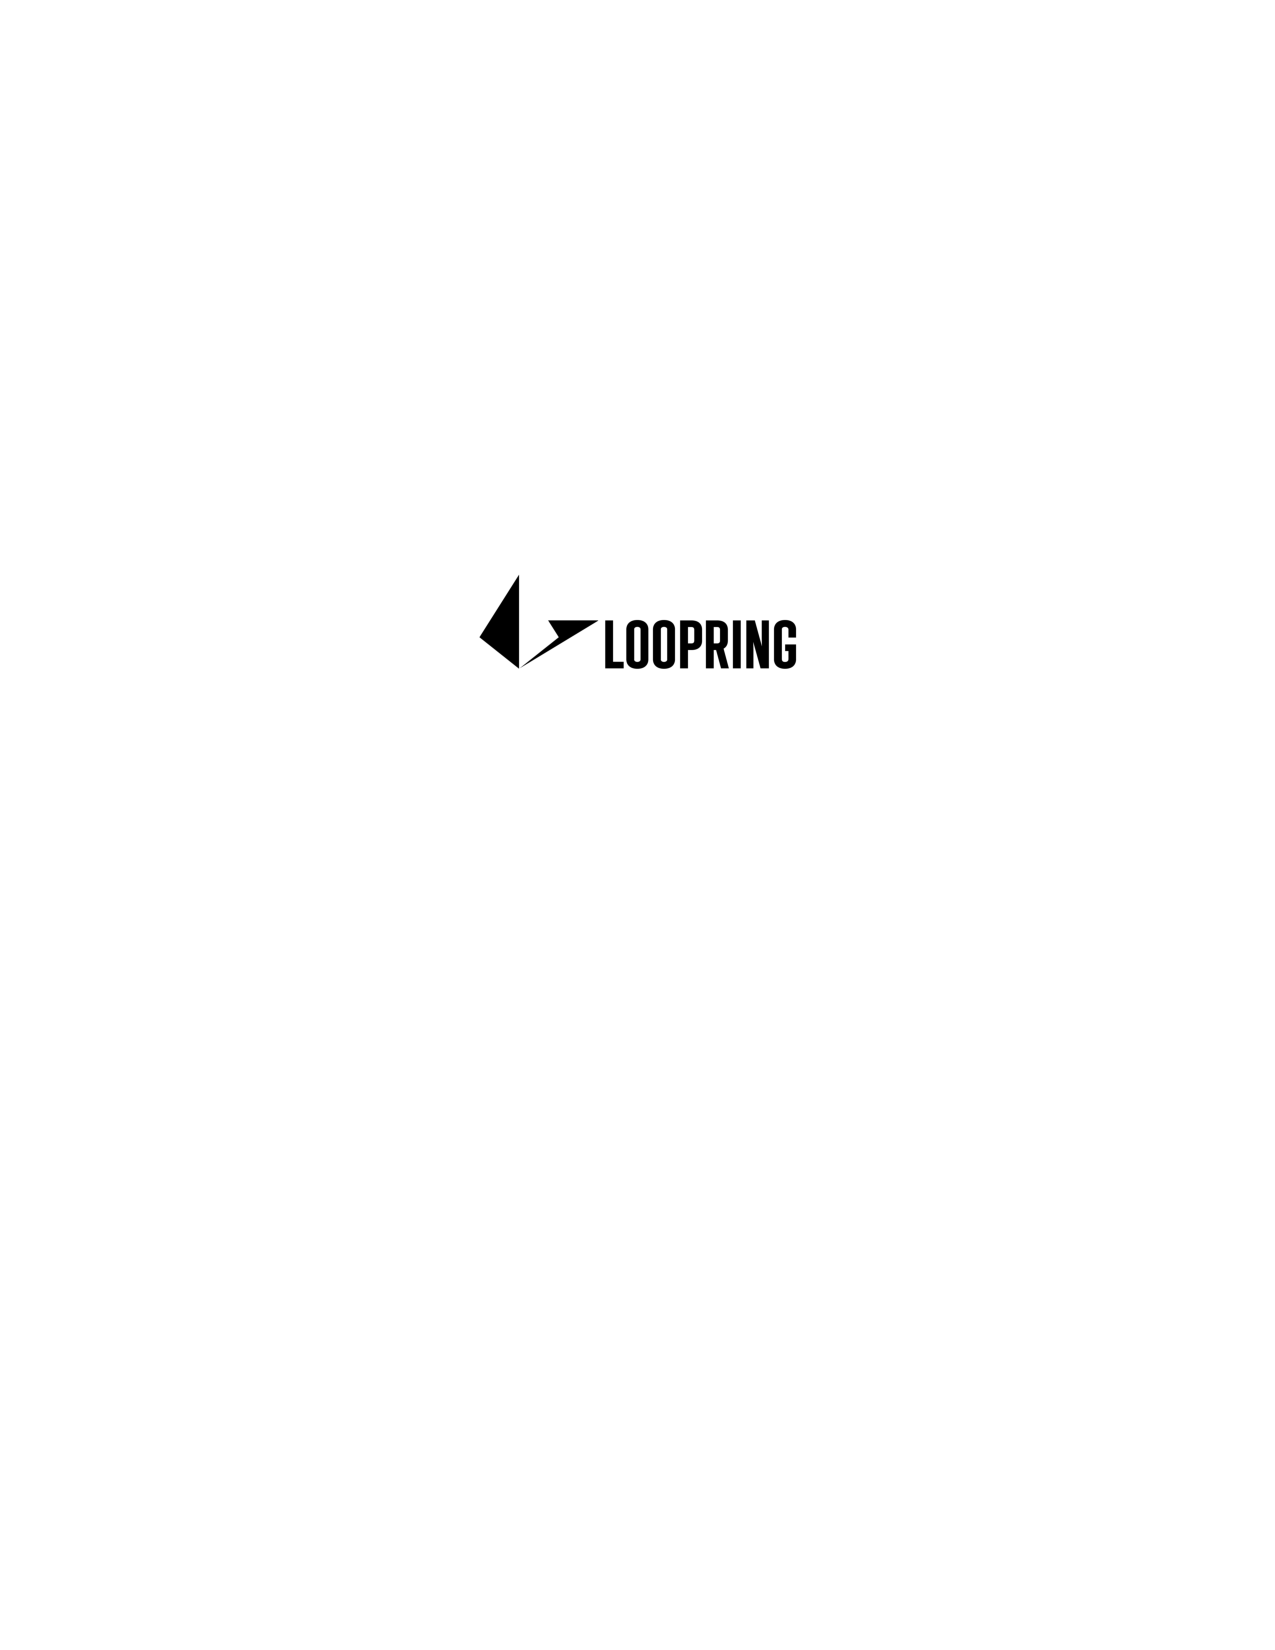
\includepdf[pages=1]{cover}
\hyphenpenalty=750


\title{\textbf{Loopring:}\\\textbf{Giao Thức Trao Đổi Phân Quyền}}
\author{
  Daniel Wang\\
  \texttt{daniel@loopring.org}\\
  \and
  	Jay Zhou\\
  	\texttt{jay@loopring.org}\\
  	\and
  	Alex Wang\\
  	\texttt{alex@loopring.org}\\
  	\and
  	Matthew Finestone\\
  	\texttt{matt.finestone@gmail.com}\\ 
  \\
  \texttt{https://loopring.org}
 }

\makeatletter
\def\CTEX@section@format{\Large\bfseries}
\makeatother

\makeatletter
\newenvironment{tablehere}
 {\def\@captype{table}}
 {}

\newenvironment{figurehere}
 {\def\@captype{figure}}
 {}
\makeatother
%
%\newcommand\BackgroundPic{%
%\put(0, 0){%
%\parbox[b][\paperheight]{\paperwidth}{%
%\vfill
%\centering
%\includegraphics[width=\paperwidth, height=\paperheight, %
%%keepaspectratio]{images/background.jpg}%
%]{images/background.jpg}%
%\vfill
%}}}


\begin{document}
%\AddToShipoutPicture{\BackgroundPic}
\maketitle


\begin{abstract}
Loopring là một giao thức mở được xây dựng nhằm tạo ra sự trao đổi phi tập trung (phân quyền). Loopring hoạt động giống như một tập hợp các hợp đồng thông minh công khai có khả năng giải quyết các giao dịch và thanh toán, với sự tập trung của các khách hàng bên ngoài chuỗi và kết nối các giao dịch với nhau. Giao thức miễn phí với người dùng, có thể mở rộng, và được sử dụng như một khối chuẩn hóa nhằm xây dựng các ứng dụng phân tán (dApps) kết hợp các chức năng giao dịch. Các tiêu chuẩn tương thích của chúng tôi giúp cho quá trình giao dịch được ẩn danh, không cần có sự tín nhiệm. Một cải tiến quan trọng so với các giao thức trao đổi phân quyền hiện nay là khả năng sắp xếp các lệnh khớp với các đơn đặt hàng khác, không giống nhau, loại bỏ các ràng buộc của hai cặp thẻ khi giao dịch và cải thiện đáng kể tính thanh khoản. Loopring cũng sử dụng một giải pháp độc đáo và mạnh mẽ để ngăn chặn hoạt động gian lận như “chạy trước”: hành động trái đạo đức khi chuyển các giao dịch thành khối dữ liệu nhanh hơn người gửi ban đầu. Loopring là chuỗi khối đa nền tảng và có thể triển khai trên bất kỳ chuỗi khối nào với chức năng hợp đồng thông minh. Vào thời điểm viết bài viết này, giao thức đã và đang hoạt động trên các nền tảng Ethereum  \cite{buterin2017ethereum} \cite{wood2014ethereum} và Qtum \cite{dai2017smart} ,đang được xây dựng trên nền tảng NEO \cite{atterlonn2018distributed} .
\end{abstract}



\begin{multicols}{2}
\section{Giới thiệu\label{sec:introduction}}

Với sự gia tăng của các tài sản số dựa trên công nghệ chuỗi khối (blockchain), nhu cầu trao đổi các tài sản này giữa các bên đã tăng đáng kể. Khi hàng ngàn loại tiền tệ số (tiền điện tử/thẻ) mới được giới thiệu bao gồm cả việc áp dụng số hóa các tài sản truyền thống - nhu cầu sử dụng loại tài sản này ngày càng gia tăng. Mặc dù việc giao dịch các loại tiền tệ số nhằm mục đích đầu cơ hay chuyển đổi để truy cập mạng lưới thông qua việc sử dụng các thẻ tiện ích gốc của họ, nhu cầu chuyển đổi các tài sản số hóa cho tài sản khác là cơ bản cho việc hình thành hệ sinh thái lớn hơn. Thực vậy, các tài sản số này cho thấy một sự tiềm năng to lớn \cite{desotocapital}, không chỉ  yêu cầu mà còn khẳng định quyền sở hữu của người dùng, mà các chuỗi khối đã cho phép bất biến, nhưng đồng thời cũng cung cấp khả năng tự do giao dịch và chuyển đổi các tài sản này.
 
Như vậy, việc giao dịch các thẻ (giá trị) mà không cần có sự tín nhiệm với các bên là một ví dụ hấp dẫn trong việc sử dụng công nghệ blockchain. Cho đến bây giờ, hầu hết những người sử dụng các tài sản số đã tiến hành giao dịch các loại tiền tệ số trên các sàn giao dịch tập trung truyền thống. Điều này càng cho chúng ta thấy giao thức Loopring là cần thiết bởi vì, giống như Bitcoin \cite{nakamoto2008bitcoin} đã từng nhấn mạnh rằng, liên quan đến giao dịch ngang hàng (peer-to-peer) tiền điện tử, \enquote{ lợi ích chính vẫn sẽ bị mất đi nếu như bên thứ ba mà người dùng tin tưởng sử dụng gian lận hai giao dịch khác nhau để cùng chi tiêu số dư của một tài khoản}, điều này cũng chính là nguyên nhân chính của sự thất thoát các tài sản tập trung nếu việc giao dịch bắt buộc phải có sự tham gia của bên thứ ba, các cổng giao dịch, các sàn giao dịch tập trung.

Theo quan điểm triết học, việc giao dịch các tài sản số phi tập trung trên các sàn giao dịch là không hề có ý nghĩa, vì các sàn giao dịch tập trung không thể đáp ứng được các đặc tính mà các dự án phi tập trung hóa mong muốn thực hiện. Ngoài ra còn có nhiều rủi ro và hạn chế thực tế trong việc sử dụng các sàn giao dịch tập trung được mô tả ở phần dưới đây. Trao đổi phi tập trung (DEXs) \cite{schuh2015bitshares} \cite{bancor} \cite{kyber} đã đưa cách giải quyết những vấn đề này, và trong nhiều trường hợp đã thành công trong việc giảm bớt rủi ro an ninh bằng cách sử dụng công nghệ chuỗi khối (blockchain) cho việc loại bỏ các bước trung gian. Tuy nhiên, trong thời gian sắp tới khả năng DEX trở thành cơ sở hạ tầng quan trọng đối với việc tạo nên nền kinh tế mới là khả thi, do đó có cần cung cấp một không gian đáng kể để cải thiện hiệu suất. Loopring hướng đến mục tiêu cung cấp các công cụ khuôn mẫu cho cơ sở hạ tầng của các dApp bằng giao thức mở bất khả tri.

\section{Bức Tranh Toàn Cảnh của Thị Trường Giao Dịch Hiện Nay\label{sec:current_exchange_landscape}}

\subsection{Những Bất Cập của Giao Dịch Tập Trung}
Ba rủi ro chính của các giao dịch tập trung là: 1) Bảo mật thấp, 2) Thiếu minh bạch, và 3) Tính thanh khoản không cao.

\textbf{Sự thiếu bảo mật} phát sinh đến từ những người tham gia, họ không kiểm soát được những mật mã (quỹ tiền) của mình. Chính điều này đã làm cho họ dễ dàng trở thành con mồi của các tin tặc trong các giao dịch của họ. Các rủi ro về an ninh và bảo mật mà các giao dịch tập trung đang phải đối mặt khá phổ biến \cite{coincheckhack}  \cite{mcmillan2014inside}, nhưng nó thường được xem như là \enquote{những khoản đặt cọc} trong giao dịch tiền tệ số. Các giao dịch này tiếp tục là những miếng mồi béo bở cho các tin tặc, bởi các tin tặc có thể dể dàng truy cập vào các máy chủ đang quản lý hàng triệu đô-la của khách hàng. Đồng thời thì các nhà phát triển cũng có thể tạo ra các lỗi ngẫu nhiên có chủ đích lên các tài khoản của khách hàng. Tóm lại thì khách hàng dường như không có khả năng kiểm soát được tài khoản của mình khi đã gửi chúng vào các sàn giao dịch.

\textbf{Sự thiếu minh bạch} sẽ làm các nhà đầu tư vướng phải nguy cơ bị lừa đảo và thiệt thòi trong chính các giao dịch của mình. Sự khác biệt ở đây là nhà đầu tư giao dịch bằng tài sản của họ có trên sàn mà là giao dịch bằng 1 IOU, điều này là một trong những mục đích không tốt của những nhà điều hành. Khi các đồng tiền được gửi vào ví, thì sàn giao dịch sẽ giữ chúng và thay thế chúng bằng IOU. Tất cả các giao dịch sẽ có hiệu lực trên các IOU của nhà đầu tư. Để thu hồi lại thì nhà đầu tư chỉ cần chuyển từ IOU sang đồng tiền, và các đồng tiền này sẽ được chuyển đến ví riêng của họ trên sàn giao dịch. Sự thiếu minh bạch trong suốt quá trình này sẽ dẫn đến hậu quả sau: giao dịch có thể bị hủy bỏ, tài khoản bị đóng băng, hoặc dẫn đến phá sản, vv … Trong khi họ cũng có thể sử dụng tài sản của nhà đầu tư với các mục đích khác, chẳng hạn như cho một bên thứ ba vay. Mặc khác, sự thiếu minh bạch có thể giúp nhà đầu tư giảm tổng chi phí trong các giao dịch như là phí giao dịch cao, chậm trễ lúc cao điểm, rủi ro về qui định và kẹt các đơn hàng trước.

\textbf{Sự thiếu tính thanh khoản.} Từ cái nhìn của những nhà điều hành, thì tính thanh khoản bị phân mảnh, nó gây ức chế lên việc tiếp cận các giao dịch mới bởi vì kịch bản là “được ăn cả, ngã về không”. Đầu tiên, giao dịch với 1 lượng tiền khổng lồ để đôi bên cùng có lợi, do vậy nhà đầu tư muốn đặt cược tất cả trong một lần giao dịch. Tiếp đó, cho đặt lệnh mua bán hàng loạt, để nhà đầu tư kiếm được lợi nhuận từ khoảng chênh lệch giữa các giao dịch. Điều này làm giảm tính cạnh tranh cho những người mới tham gia vì rất khó để họ thanh khoản chi phí ban đầu. Kết quả là nhiều giao dịch đòi hỏi thị phần cao, mặc dù đã có sự phàn nàn từ phía nhà đầu tư và thậm chí có những cuộc tấn công lớn từ tin tặc. Cần lưu ý rằng, thị trường càng béo bở thì nó càng dễ trở thành mục tiêu đáng chú ý cho tin tặc.

Từ quan điểm của nhà đầu tư, tính thanh khoản bị phân mảnh làm giảm đáng kể trải nghiệm của nhà đầu tư. Trong một giao dịch đơn cử, nhà đầu tư chỉ giao dịch được với các đồng mà sàn giao dịch này cung cấp, với các lệnh mua bán và những đồng có tính thanh khoản hỗ trợ cho các đồng của sàn giao dịch đó. Để mà chuyển đổi từ đồng \verb|A| sang đồng \verb|B|, nhà đầu tư phải tìm đến một sàn giao dịch trung gian có hỗ trợ 2 đồng đó và nhà đầu tư phải đăng kí thông tin tại sàn trung gian đó đồng nghĩa với lại việc tiết lộ các thông tin cá nhân của mình. Nhà đầu tư thường phải thực hiện các bước cơ bản hoặc trung gian, thông qua các đồng BTC hoặc ETH và phải trả phí cho quá trình đó. Cuối cùng thì, những lệnh đặt trước thường không đủ mạnh để có thể giao dịch thành công mà không có sự hao tổn. Ngay cả khi có sự hỗ trợ cho một lượng giao dịch khổng lồ thì cũng không có gì đảm bảo rằng khối lượng và tính thanh khoản đó không phải là giả \cite{fakevolume}. 

Kết quả là tính thanh khoản bị phá vỡ và một hệ sinh thái bị phân mảnh tương tự như một hệ thống tài chính dư thừa, với một khối lượng đáng kể tập trung tại một số giao dịch. Các cam kết thanh khoản của chuỗi khối không có giá trị trong các giao dịch này.

\subsection{Những Hạn Chế Trong Việc Giao Dịch Phi Tập Trung}
Các giao dịch phi tập trung khác với các giao dịch tập trung một phần, bởi vì nhà đầu tư duy trì sự kiểm soát của mình lên các mã cá nhân (tài sản) bằng cách thực hiện các giao dịch trực tiếp trên qua mạng lưới chuỗi khối. Bằng việc giảm tin tưởng vào các công nghệ của các đồng tiền điện tử, họ đã giảm thiểu nhiều rủi ro về các vấn đề bảo mật. Tuy nhiên, sự hiệu quả và cơ cấu hạn chế vẫn còn tồn tại nhiều vấn đề. 

Thanh khoản vẫn là vấn đề vì nhà đầu tư phải tìm kiếm các đối tác chấp nhận các khoản thanh khoản và tiêu chuẩn thanh khoản tương đối. Các hiệu ứng thanh khoản vẫn tồn tại nếu như DEXs hoặc dApps không sử dụng các tiêu chuẩn chung để tương tác và nếu các đơn hàng không được chia sẻ hoặc tuyên truyền rộng rãi trên một mạng lưới. Tính thanh khoản của các lệnh đặt trước và cụ thể là khả năng phục hồi của chúng – có thể ảnh hưởng lớn tới các chiến lược kinh doanh tối ưu \cite{limitorderliquidity}. Không có các tiêu chuẩn rõ ràng không chỉ dẫn đến việc giảm thanh khoản mà còn liên quan đến hàng loạt các hợp đồng thông minh không an toàn.

Hơn nữa, kể từ khi các giao dịch được thực hiện ở dạng chuỗi, DEXs đã kế thừa những hạn chế của blockchain, cụ thể là:  sự chậm trễ trong việc thực hiện (đào coin), và tốn kém chi phí trong việc thay đổi đặt lệnh mua bán. Do đó, việc đặt lệnh trước vào chuỗi khối không thực sự tốt, vì khi thực hiện các lệnh trên blockchain bạn phải chịu một chi phí (chi phí hoạt động), làm cho các lệnh hủy trở nên phức tạp và rất tốn kém. 

Cuối cùng do các lệnh đặt trước ở blockchain được công khai nên các thợ đào có thể nhìn thấy các đơn hàng thì điều đó có nghĩa là các thợ mỏ sẽ khai thác ở lần tiếp theo để cung cấp cho đơn hàng đó. Sự chậm trễ này có thể làm cho nhà đầu tư chịu rủi ro bị hớt tay trên và phải chịu những cái giá hoặc giao dịch bất lợi về phía mình.

\subsection{Các Giải Pháp Lai}
Vì những lý do nêu trên, nên những sàn giao dịch dựa trên công nghệ chuỗi khối có những hạn chế mà làm cho chúng không cạnh tranh được với các sàn tập trung. Có một sự đánh đổi giữa việc không cần có sự tín nhiệm vào bất kì người nào trong chuỗi và việc tốc độ và độ linh hoạt của sàn tập trung. Những giao thức như Loopring và 0x \cite{warren20170x} mở rộng giải pháp giải quyết trên chuỗi và quản lý lệnh ngoài chuỗi. Các giải pháp này xoay quanh hợp đồng thông minh mở, nhưng thông qua sự giới hạn mở rộng bằng cách thực hiện một số chức năng ngoài chuỗi và cho thêm nodes sự linh hoạt trong hoàn thành vai trò quan trọng đối với mạng lưới. Tuy nhiên, mô hình Lai vẫn còn một số nhược điểm \cite{costofdecent}. Giao thức Loopring đề xuất những khác biệt có ý nghĩa đáng kể trong cách tiếp cận giải pháp lai được mô tả trong bài viết này.


\section{Giao Thức Loopring\label{sec:loopring_protocol}}
Loopring không phải là sàn giao dịch phi tập trung (DEX), nhưng là một giao thức khuôn mẫu để xây dựng các giao dịch phi tập trung trên nhiều chuỗi khối. Chúng tôi loại bỏ các thành phần không cần thiết trong các giao dịch truyền thống và đưa ra một bộ hợp đồng thông minh công khai và . Các thành phần đóng vai trò trong mạng lưới bao gồm ví, rơ-le, chia sẻ thanh khoản, các trình duyệt hỗ trợ việc đặt lệnh, các thợ đào trong chu trình và các dịch vụ số hóa (thẻ) tài sản. Nhưng trước khi định nghĩa từng thành phần, chúng ta nên hiểu được việc đặt lệnh trong Loopring là như thế nào. 

\subsection{Chu Trình Giao Dịch\label{sec:order_ring}}
Các trao đổi trong Loopring được thể hiện dựa trên mô hình chúng tôi gọi là ”mô hình giao dịch một chiều” (UDOM)\cite{coinport2014udom}. UDOM thể hiện lệnh như yêu cầu trao đổi thẻ, \verb|lượngS|/\verb|lượngB|, (lượng thẻ bán ra/mua vào) thay vì đặt tỷ giá và đấu giá. Vì mỗi lệnh mua bán chỉ là một tỷ giá hối đoái giữa hai thẻ do đó một tính năng mạnh mẽ mới của giao thức là sự pha trộn và kết hợp của nhiều đơn đặt hàng trong một vòng giao dịch. Bằng cách sử dụng lên đến 16 đơn đặt hàng thay vì một cặp giao dịch duy nhất, đó là một sự gia tăng đáng kể trong tính thanh khoản và khả năng để cải thiện giá. 

\begin{center}
\begin{figurehere}
\centering
\tikzstyle{block} = [draw, fill=blue!20, rectangle, 
    minimum height=3em, minimum width=6em]
\tikzstyle{sum} = [draw, fill=blue!20, circle, node distance=1cm]
\tikzstyle{input} = [coordinate]
\tikzstyle{output} = [coordinate]
\tikzstyle{pinstyle} = [pin edge={to-,thin,black}]

\begin{tikzpicture}[
    auto, 
    node distance=2cm,
    >=latex',
    font=\bfseries\footnotesize\sffamily,
    order/.style={
		scale=0.7,
		rectangle,
		rounded corners,
		draw=black, 
		text centered,
%		text width=5cm,
		minimum height=12mm,
		fill=white
	},
	label/.style={
		scale=0.7
	}
  ]
    % We start by placing the blocks

  \node [order] (order2) 
 {%
 \begin{tabular}{l}
  \textbf{LỆNH\#2}\\
  \textbf{người dùng: Y}\\
  \textbf{lượngS: 9B}\\
  \textbf{lượngB: 12C}
 \end{tabular}
 };
 
  \node [order, below of=order2, xshift=-3.5cm] (order1) 
 {%
 \begin{tabular}{l}
  \textbf{LỆNH\#1}\\
  \textbf{người dùng: X}\\
  \textbf{lượngS: 10000A}\\
  \textbf{lượngB: 2B}
 \end{tabular}
 };
 
 
  \node [order, below of=order2, xshift=3.5cm] (order3) 
 {%
 \begin{tabular}{l}
  \textbf{LỆNH\#3}\\
  \textbf{người dùng: Z}\\
  \textbf{lượngS: 100C}\\
  \textbf{lượngB: 160A}
 \end{tabular}
 };
 
 \draw [draw,->] (order1) -- node [label] {\textbf{7898A}} (order3);
 \draw [draw,->] (order2) -| node [label, xshift=-1.8cm] {\textbf{8B}} (order1);
 \draw [draw,->] (order3) |- node [label, xshift=1cm, yshift=0.24cm] {\textbf{98C}} (order2);

\end{tikzpicture}

\caption{Một chu trình trao đổi của 3 lệnh khác nhau}
\label{fig:ring}
\end{figurehere}
\end{center}


Hình trên cho thấy một chu trình mua bán gồm 3 lệnh được đưa ra. Mã thông báo của mỗi đơn đặt hàng để bán (\verb|thẻS|) là mã thông báo của một đơn đặt hàng khác để mua (\verb|thẻB|). Điều này tạo ra một vòng lặp cho phép các lệnh đưa ra có thể trao đổi các thẻ mong muốn mà không đòi hỏi cần có sự xuất hiện của một lệnh đối lập với nó. Các cặp lệnh giao dịch truyền thống vẫn có thể, dĩ nhiên, vẫn được thực hiện, về cơ bản, nó chỉ là 1 trường hợp đặc biệt trong chu trình lệnh. 

\begin{definition}[Chu trình lệnh] Gọi $C_{0}$, $C_{1}$, $\cdots$, $C_{n-1}$ là $n$ thẻ khác nhau, $O_{0\rightarrow 1}$, $\cdots$, $O_{i\rightarrow i\oplus 1}$, $\cdots$, $O_{n-1 \rightarrow 0}$ là $n$ lệnh. Các lệnh này sẽ được biểu diễn thành 1 chu trình lệnh để trao đổi như sau:
$$O_{0\rightarrow 1} \rightarrow \cdots \rightarrow O_{i\rightarrow i\oplus 1} \rightarrow \cdots \rightarrow O_{n-1\rightarrow 0} \text{, }$$
trong đó $n$ là độ dài của chu trình lệnh, và $i\oplus 1 \equiv i+1 \mod n$.
\end{definition}

Một chu trình mua bán có giá trị (hiệu lực) khi tất cả các thành phần giao dịch được thực hiện với tỷ giá hối đoái bằng hoặc cao hơn giá gốc ban đầu được xác định ngầm định bởi người dùng. Để xác minh tính hiệu lực của lệnh được đưa ra, các hợp đồng thông minh sử dụng giao thức Loopring phải nhận được các lệnh mua bán được gửi từ các thợ đào trong chính chu trình nơi mà sản phẩm của tỷ giá hối đoái ban đầu của tất cả các lệnh bằng hoặc lớn hơn 1.

Giả sử Alice và Bob muốn giao dịch các thẻ của họ là thẻ \verb|A| và thẻ \verb|B|. Alice có 15 thẻ \verb|A| và cô ấy muốn đổi chúng lấy 4 thẻ \verb|B|; Bob có 10 thẻ \verb|B| và anh ta muốn có được 30 thẻ \verb|A| từ số thẻ trên.

Ai là người mua và ai là người bán? Điều này chỉ phụ thuộc vào số tài sản mà chúng tôi dùng để cố định giá trị trên bảng báo giá. Nếu sử dụng thẻ \verb|A| là số liệu tham chiếu, thì Alice đang mua thẻ \verb|B| với giá là  ${15 \over 4} = 3.75$\verb|A|, trong khi đó Bob đang bán 10 thẻ \verb|B| với giá ${30 \over 10} = 3.00$\verb|A|. Trong trường hợp lấy thẻ B là số liệu tham chiếu, chúng tôi nói rằng Alice đang bán 15 thẻ \verb|A| cho giá là ${4\over 15}=0.26666667$\verb|B| và Bob đang mua 10 thẻ \verb|A| với giá là ${10 \over 30}=0.33333334$\verb|B|. Do đó, ai là người mua hoặc người bán vẫn còn phải tùy thuộc vào từng trường hợp.

Trong tình huống đầu tiên, Alice sẵn sàng trả giá cao hơn ($3.75$\verb|A|) so với giá mà Bob đang bán thẻ của mình ($3.00$\verb|A|), trong khi trong trường hợp thứ hai Bob sẵn sàng trả giá cao hơn ($0.33333334$\verb|B|) so với giá Alice đang bán thẻ của cô ấy ($0.26666667$\verb|B|). Rõ ràng là việc trao đổi mua bán có thể xảy ra bất cứ khi nào người mua sẵn sàng trả giá bằng hoặc cao hơn giá của người bán.

\begin{equation}
{{15\over 4} \over {30\over 10}} = {{10\over 30} \over {4\over 15}}={15 \over 4} \cdot {10 \over 30} = 1.25 > 1
\end{equation}

Do đó, để xác định việc đưa ra tập hợp n lệnh đưa ra có được giải quyết hoàn toàn hay một một phần, chúng ta cần phải biết liệu tỷ giá hối đoái cho từng sản phẩm giống như giá trị mà lệnh mua đưa ra có lớn hơn hay bằng 1 hay không. Nếu có, tất cả n lệnh giao dịch đưa ra có thể được giải quyết một phần hoặc hoàn toàn giải quyết \cite{supersymmetry}.

Nếu chúng ta giới thiệu thêm một đối tác thứ ba là Charlie, như vậy Alice muốn bán ra một lượng $x_1$ thẻ \verb|A| và nhận được một lượng $y_1$ thẻ \verb|B|, Bob muốn bán ra một lượng $x_2$ thẻ \verb|B| và muốn có được lượng $y_2$ thẻ \verb|C|, và Charlie muốn trao đổi số lượng $x_3$ thẻ \verb|C| để đổi lấy lượng $y_3$ thẻ \verb|A|. Điều cần thiết ở đây là lượng thẻ bán ra của các bên đều là có thật, và giao dịch có thể được thực hiện nếu:

\begin{equation}
{{x_1 \cdot x_2 \cdot x_3 \over y_1 \cdot y_2 \cdot y_3} \geq 1}
\end{equation}


Xem phần \ref{anatomy} để biết thêm chi tiết về các lệnh mua bán trong Loopring.



\section{Những Người Tham Gia Hệ Sinh Thái\label{sec:ecosystem}}
Tất cả mọi người tham gia hệ sinh thái của Loopring đều được cung cấp đầy đủ các công cụ giống như một sàn trao đổi tập trung đã đưa ra. 

\begin{itemize}

\item \textbf{Ví tiền}: Một dịch vụ ví hoặc giao diện thông thường có khả năng cho phép người dùng truy cập các thẻ của họ và cách gửi lệnh mua bán/trao đổi tới mạng lưới Loopring. Ví tiền sẽ được khuyến khích sử dụng để đưa ra các lệnh trao đổi bằng cách chia sẻ các khoản phí với các thợ đào trong chu trình(xem phần\ref{sec:token}). Với niềm tin rằng tương lai của việc giao dịch sẽ an toàn khi người dùng sử dụng ví cá nhân của họ, việc kết nối các nhà cung cấp thanh khoản này thông qua giao thức của chúng tôi là vô cùng quan trọng.

\item \textbf{Chia Sẻ Thanh Khoản Trong Liên Kết Chuỗi Khối/ Rơ-le Vô Tuyến}: Một mạng lưới chuyển tiếp vô tuyến và khả năng chia sẻ tính thanh khoản. Khi các nút chạy phần mềm chuyển tiếp Loopring, chúng có thể tham gia vào một mạng lưới hiện có và chia sẻ thanh khoản với các rơ-le (nút chuyển tiếp) khác qua sự liên kết giữa các chuỗi khối. Sự liên kết trong chuỗi khối mà chúng tôi đang xây dựng như là một sự hoàn thành đầu tiên có khả năng chia sẻ lệnh gần với thời gian thực (1-2 giây khối), và loại bỏ các lịch sử cũ để cho phép tải nhanh hơn bởi các nút mới. Điều đáng chú ý ở đây, các nút chuyển tiếp không cần phải tham gia vào sự liên kết này; chúng có thể hoạt động riêng rẽ và không cần chia sẻ tính thanh khoản với các nút khác hoặc có thể tự tạo ra và quản lý mạng lưới chia sẻ thanh khoản của chính chúng.

\item \textbf{Rơ-le/Thợ Đào Trong Chu Trình}: Rơle (nút chuyển tiếp) là các nút nhận các lệnh từ ví hoặc các nút chuyển tiếp vô tuyến, có nhiệm vụ duy trì đơn lệnh mua bán công khai đã được đưa ra và lịch sử giao dịch, và tùy chọn gửi các lệnh mua bán cho các rơ-le khác (thông qua bất kỳ các kênh ngoại tuyến nào) và / hoặc nút chuyển tiếp vô tuyến. Việc khai thác (đào) trong chu trình là một tính năng – không phải là điều bắt buộc đối với các nút chuyển tiếp. Đây là một việc thiên về tính toán và được thực hiện hoàn toàn ngoài chuỗi. Chúng tôi gọi những người có thể kích hoạt các tính năng đào trong chu trình đối các rơ-le là \enquote{Thợ đào trong chu trình}, người thực hiện các lệnh mua bán trong chu trình bằng cách ghép các đơn đặt hàng khác nhau. Các nút chuyển tiếp được tự do trong việc (1) làm thế nào chúng có thể kết nối với nhau, (2) cách chúng xây dựng các lệnh mua bán được đưa ra, và (3) làm thế nào chúng khai thác được những lệnh mua bán trong chu trình (thuật toán khai thác mỏ).

\item \textbf{Giao Thức Hợp Đồng Thông Minh Loopring (LPSC)}: Một nhóm các hợp đồng thông minh được công khai và sử dụng miễn phí nhằm kiểm tra các lệnh trong chu trình từ các thợ đào, giúp giải quyết các giao dịch không cần có sự tín nhiệm và chuyển giao thẻ (token) trên danh nghĩa người dùng, khuyến khích các thợ đào cũng như các dịch vụ ví điện tử bằng cách trả phí và tạo ra nhiều sự kiện. Rơle hay các trình duyệt mua bán luôn theo dõi những các hoạt động này để cập nhật kịp thời các lệnh mua bán được đưa ra cũng như lịch sử giao dịch. Xem phụ lục \ref{app:protocol_ethereum} để biết chi tiết.

\item \textbf{Dịch Vụ Số (thẻ) Hóa Tài Sản (ATS)}: Đây là một cầu nối cho các loại tài sản không thể giao dịch trực tiếp trên mạng lưới của Loopring và là các dịch vụ tập trung do các công ty hoặc tổ chức đáng tin cậy điều hành. Người dùng gửi tài sản (thực, fiat hoặc mã thông báo từ các chuỗi khác) và nhận lại các thẻ (token) có giá trị tương đương, có thể được sử dụng để đặt cọc trong tương lai. Loopring không phải là giao thức có thể trao đổi chéo (cho đến khi có giải pháp phù hợp), nhưng dịch vụ ATS cho pép người dùng trao đổi các thẻ chạy trên nền tảng ERC20 \cite{ERC20} với tài sản mang ý nghĩa vật chất cũng như tài sản được tạo ra từ các công nghệ chuỗi khối khác. 

\end{itemize}


\section{Quy Trình Trao Đổi\label{sec:process}}



\begin{enumerate} 


\item \textbf{Ủy Quyền Giao Thức}: Trong hình \ref{fig:process}, người dùng \verb|Y| muốn giao dịch số thẻ thông qua việc ủy quyền cho LPSC xử lý một \verb|lượngS| của thẻ \verb|B| mà người dùng muốn bán. Việc ủy quyền cho giao thức này số lượng thẻ mà người dùng muốn bán sẽ không bị khóa, người dùng vẫn có thể tự do di chuyển chúng trong khi lệnh trao đổi vẫn đang được thực hiện.

\item \textbf{Tạo Lệnh}: Tỉ giá hiện tại và việc tiến hành đặt lệnh mua bán cho hai loại thẻ \verb|B| và \verb|C| được cung cấp bởi các rơ-le hoặc các các đại lý được kết nối với mạng lưới, chẳng hạn như các trình duyệt dùng để đặt lệnh trao đổi. Người dùng \verb|Y| có thể đưa ra lệnh trao đổi (lệnh có giới hạn) với \verb|lượngS| và \verb|lượngB| cụ thể cũng như các yếu tố khác thông qua bất kì ví điện tử có tích hợp. Một lượng thẻ LRx có thể được thêm vào và được dùng để làm chi phí chi trả cho các thợ đào trong chu trình; lượng phí LRx người dùng trả càng cao thì cơ hội để lệnh mua bán được xử lí càng nhanh hơn. Mã băm (hash) của lệnh được xác nhận với mã cá nhân của người dùng \verb|Y|.

\begin{center}
\begin{figurehere}
\centering
\tikzstyle{block} = [draw, fill=blue!20, rectangle, 
    minimum height=3em, minimum width=6em]
\tikzstyle{sum} = [draw, fill=blue!20, circle, node distance=1cm]
\tikzstyle{input} = [coordinate]
\tikzstyle{output} = [coordinate]
\tikzstyle{pinstyle} = [pin edge={to-,thin,black}]

\begin{tikzpicture}[
    auto, 
    scale=0.7,
    node distance=2cm,
    >=latex',
    font=\bfseries\footnotesize\sffamily,
    order/.style={
		rectangle,
		scale=0.7,
		rounded corners,
		draw=black, 
		text centered,
%		text width=5cm,
		minimum height=12mm,
		minimum width=30mm,
		fill=white
	},
	role/.style={
		circle,
		scale=0.7,
		draw=black, 
		text centered,
%		text width=5cm,
		minimum height=12mm,
		minimum width=12mm,
		fill=white
	},
	steps/.style={
		circle,
		scale=0.7,
		draw=black, 
		text centered,
%		text width=5cm,
%		minimum height=12mm,
%		minimum width=12mm,
		fill=black,
		text=white
	},
	account/.style={
		circle,
		scale=0.7,
		draw=black, 
		text centered,
%		text width=5cm,
		minimum height=16mm,
		minimum width=16mm,
		fill=white
	},
	label/.style={
	  scale=0.7
    }
  ]

 
 \node [role] (user1)  {Người dùng X};
 \node [role, below of=user1] (user2)  {Người dùng Y};
 \node [role, below of=user2] (user3)  {Người dùng Z};
 \node [role, below of=user3, fill=gray!20] (relay1)  {Rơ-le M};
 \node [role, below of=relay1, fill=gray!20] (relay2)  {Rơ-le N};

 
 \node [order, left of=user1, xshift=-1cm] (order1) 
 {%
 \begin{tabular}{l}
  \textbf{LỆNH\#1}\\
  \textbf{người sở hữu: X}\\
  \textbf{lượngS: 10000 A}\\
  \textbf{lượngB: 2 B}
 \end{tabular}
 };
 
 \draw [draw, ->]  (user1) -- (order1) [label]{};
 \draw [bend right,->] (order1) to node [auto, scale=0.7] {} (relay1);
 \draw [bend right,->] (order1) to node [auto, scale=0.7] {} (relay2);
% \draw [draw, ->]  (order1) |- (relay1) [label]{};
% \draw [draw, ->]  (order1) |- (relay2) [label]{};
 
 \node [order,left of=user2, xshift=-1.5cm] (order2) 
 {%
 \begin{tabular}{l}
  \textbf{LỆNH\#2}\\
  \textbf{người sở hữu: Y}\\
  \textbf{lượngS: 9  B}\\
  \textbf{lượngB: 12 C}
 \end{tabular}
 };
 \draw [draw, ->]  (user2) -- (order2) [label]{};
 \draw [bend right,->] (order2) to node [auto, scale=0.7] {} (relay1);
 \draw [bend right,->] (order2) to node [auto, scale=0.7] {} (relay2);
% \draw [draw, ->]  (order2) |- (relay1) [label]{};
% \draw [draw, ->]  (order2) |- (relay2) [label]{};
% 
\node [order, left of=user3, xshift=-2cm] (order3) 
 {%
 \begin{tabular}{l}
  \textbf{LỆNH\#3}\\
  \textbf{người sở hữu: Z}\\
  \textbf{lượngS: 100 C}\\
  \textbf{lượngB: 160 A}
 \end{tabular}
 };
 \draw [draw, ->]  (user3) -- (order3) [label]{};
 \draw [bend right,->] (order3) to node [auto, scale=0.7] {} (relay1);
 \draw [bend right,->] (order3) to node [auto, scale=0.7] {} (relay2);
% \draw [draw, ->]  (order3) |- (relay1) [label]{};
% \draw [draw, ->]  (order3) |- (relay2) [label]{};
 
% // The Ring
\node [order, 
yshift=-1.5cm,
xshift=-2.75cm,
below of=relay2,
fill=gray!10,
minimum width=4.2cm,
minimum height=5cm] (ring) {};


\node [order, dashed, below of=relay2,yshift=-0.2cm,xshift=-2.5cm] (order11) 
 {%
 \begin{tabular}{l}
  \textbf{LỆNH\#1}\\
  \textbf{người sở hữu: X}\\
  \textbf{lượngS: 10000 A}\\
  \textbf{lượngB: 2 B}
 \end{tabular}
 };
 \node [order, dashed,below of=order11,xshift=-0.25cm,yshift=0.7cm] (order21) 
 {%
 \begin{tabular}{l}
  \textbf{LỆNH\#2}\\
  \textbf{người sở hữu: Y}\\
  \textbf{lượngS: 9  B}\\
  \textbf{lượngB: 12 C}
 \end{tabular}
 };
\node [order, dashed,below of=order21,xshift=-0.25cm,yshift=0.7cm] (order31) 
 {%
 \begin{tabular}{l}
  \textbf{LỆNH\#3}\\
  \textbf{người sở hữ: Z}\\
  \textbf{lượngS: 100 C}\\
  \textbf{lượngB: 160 A}
 \end{tabular}
 };
 
 % // The blockchain
\node [
rectangle,
fill=gray!20, 
right of=user1,
yshift=-4.5cm,
xshift=0.1cm,
scale=0.7,
minimum width=3.2cm,
minimum height=15.6cm] (blockchain) {\parbox[b][15cm]{1.3cm}{Chuỗi khối}};
% blockchain accounts
  \node [account, right of=user1, xshift=1cm] (account1)  {Tài khoản X};
  \node [account, right of=user2, xshift=1cm] (account2)  {Tài khoản Y};
  \node [account, right of=user3, xshift=1cm] (account3)  {Tài khoản Z};
  \node [account, right of=relay1, xshift=1cm] (account4)  {Tài khoản M};
  \node [account, right of=relay2, xshift=1cm] (account5)  {Tài khoản N};
  \node [account, double, below of=account5, yshift=-1.5cm] (psc)  {LPSC};
  
 \draw [draw, ->]  (user1) -- (account1) [label]{};
 \draw [draw, ->]  (user2) -- (account2) [label]{};
 \draw [draw, ->]  (user3) -- (account3) [label]{};
% \draw [draw, ->]  (relay1) -- (account4) [label]{};
% \draw [draw, ->]  (relay2) -- (account5) [label]{};
 \draw [draw, double, thick]  (relay1) to node [auto, scale=0.7] {Chia sẻ thanh khoản}  (relay2) [label]{};
% \draw [draw, ->]  (relay1) -- (ring) [label]{};
 \draw [draw, ->]  (relay2) to node [auto, scale=0.7, xshift=-1.8cm, yshift=0.3cm] {Chu trình khai thác}  (ring) [label]{};
 \draw [draw, ->]  (ring) to node [auto, scale=0.7] {Xác nhận chu trình} (psc) [label]{};
 
 \draw [bend left,->] (account1) to node [auto, scale=0.7] {\textbf{7898 A}} (account3);
 \draw [bend left,->] (account2) to node [auto, scale=0.7] {\textbf{8 B}} (account1);
 \draw [bend left,->] (account3) to node [auto, scale=0.7] {\textbf{98 C}} (account2);
 
 \draw [bend left,->, dashed] (account1) to node [auto, scale=0.7] {} (account5);
 \draw [bend left,->, dashed] (account2) to node [auto, scale=0.7] {} (account5);
 \draw [bend left,->, dashed] (account3) to node [auto, scale=0.7, xshift=.5cm] {\textbf{Chi phí}} (account5);
  
  
% \draw [draw,->] (order1) -- node [label] {\textbf{7898 A}} (order3);
% \draw [draw,->] (order2) -| node [label, xshift=-1.8cm] {\textbf{8 B}} (order1);
% \draw [draw,->] (order3) |- node [label, xshift=1cm, yshift=0.24cm] {\textbf{98 C}} (order2);

\node [steps, right of=user2, xshift=-0.6cm] () {1};
\node [steps, left of=user2, xshift=0.8cm] () {2};
\node [steps, left of=relay2, xshift=0.3cm, yshift=1cm] () {3};
\node [steps, left of=relay1, xshift=3.3cm, yshift=-1.6cm] () {4};
\node [steps, below of=relay2, xshift=-0.2cm, yshift=0.4cm] () {5};
\node [steps, right of=account3, xshift=-0.6cm] (step5) {6};

 \draw [bend right, ->]  (psc) to node [auto, scale=0.7, xshift=0.5cm] {Thanh toán} (step5) [label]{};
 
\end{tikzpicture}

\caption{Quy trình trao đổi Loopring}
\label{fig:process}
\end{figurehere}
\end{center}


\item \textbf{Truyền Lệnh}: Lệnh trao đổi cũng như mã xác nhận của chúng sẽ được ví điện tử gửi đến một hoặc nhiều rơ-le. Các rơ-le sẽ tiến hành cập nhật danh sách lệnh trao đổi công khai. Giao thức không yêu cầu các danh sách lệnh trao đổi phải được xây dựng theo một cách xác định, giống như ai đến trước sẽ được ưu tiên phục vụ trước. Thay vào đó, các rơ-le có quyền tự thiết kế quyết định của chúng trong việc thực hiện danh sách các lệnh mua bán.

\item \textbf{Chia Sẻ Thanh Khoản}: Các rơ-le truyền các lệnh giao dịch tới các rơ-le khác thông qua bất kỳ các phương tiện truyền thông nào. Một lần nữa cho chúng ta thấy được sự linh hoạt thông qua cách mà các nút tương tác với nhau. Để tạo điều kiện cho mức độ nhất định của kết nối mạng, chúng tôi xây dựng việc chia sẻ tính thanh khoản thông qua mạng lưới rơ-le bằng cách sử dụng một tổ hợp chuỗi khối. Như đã đề cập trong phần trước, các rơ-le vô tuyến này được sử dụng để tối ưu hóa cho tốc độ và độ phủ sóng.

\item \textbf{Chu Trình Đào (Sự Khớp Lệnh)}:  Các thợ đào cố gắng hoàn thành toàn bộ hoặc một phần lệnh giao dịch đưa ra tại tỷ giá hối đoái hoặc tốt hơn bằng cách bắt cặp chúng với nhiều lệnh khác. Chu trình khai thác là nguyên nhân chính cho việc tại sao giao thức cho phép cung cấp tính thanh khoản cao trên bất kì cặp giao dịch nào. Nếu tỷ lệ thực hiện tốt hơn so với những gì người dùng \verb|Y| đã chỉ định, thì số tiền ký quỹ được chia sẻ giữa tất cả các lệnh trao đổi trong chu trình. Như một phần thưởng, người thợ đào sẽ lựa chọn giữa việc yêu cầu một phần lợi nhuận (chia phần tiền ký quỹ, và trả lại LRx cho người dùng), hoặc đơn giản là giữ LRx làm chi phí.

\item \textbf{Xác Thực\& Thanh Toán}: Chu trình xử lý lệnh mua bán được thực hiện bở LPSC. Quá trình này trải qua hàng loạt các bước kiểm tra nhằm xác thực các dữ liệu được cung cấp bởi các thợ đào và xác định rằng liệu có thể giải quyết hoàn toàn hay một phần các lệnh này ( phụ thuộc vào tốc độ điền thông tin của lệnh vào trong chu trình và lượng thẻ có trong ví của người dùng). Nếu tất cả các bước kiểm tra đều được thông qua, hợp đồng thông minh sẽ tự động chuyển đổi các thẻ giữa các bên người dùng và chi trả chi phí cho thợ đào cũng như của ví trong cùng một thời điểm. Nếu số dư của người dùng \verb|Y| được xác định bởi LPSC là không đủ, giao dịch sẽ được thu nhỏ lại: giao dịch sẽ tiếp tục được thực hiện (mở rộng đến kích thước ban đầu) khi lượng thẻ không đủ được bổ sung vào địa chỉ ban đầu, không giống như việc hủy bỏ lệnh, được thực hiện thủ công và không thể đảo ngược.


\end{enumerate}





%
%\end{multicols}
%
%\begin{center}
%\begin{figurehere}
%\includegraphics[height=8cm]{images/en_protocol.png}
%\caption{Loopring Trading Process}
%\label{fig: Loopringrotocol}
%\end{figurehere}
%\end{center}
%
%\begin{multicols}{2}

\section{Sự Linh Hoạt Trong Cách Thức Hoạt Động\label{sec:business_model}}
Có một điều quan trọng cần chú ý ở đây rằng Loopring cho phép người tham gia có sự linh hoạt đáng kể trong việc mở ra các hoạt động của chính họ. Người dùng được tự do triển khai các mô hình kinh doanh mới, mang lại lợi nhuận cho chính họ cũng như kiếm được kinh phí từ các thẻ LRx dựa trên thành quả công việc cũng như những thước đo khác trong quá trình hoạt động (nếu họ chọn). Hệ sinh thái của Loopring cũng cung cấp những khuôn mẫu và các giá trị trung bình nhằm hỗ trợ người tham gia thông qua rất nhiều các ứng dụng khác nhau.


\subsection{Sổ Lệnh\label{sec:order_book}}
Các cảm biến có thể thiết kế sổ lệnh của họ theo rất nhiều cách để hiển thị và khớp các lệnh của người đặt lệnh. Sổ lệnh đầu tiên của chúng ta triển khai theo một như mô hình OTC, nơi mà những lệnh giới hạn được định giá dựa trên đơn giá. Timestamps (Biểu thị thời gian) của lệnh, hay nói cách khác, chẳng hề liên quan gì đến sổ lệnh. Tuy nhiên, các cảm biến tự do thiết kế sổ lệnh của họ sao cho mô phỏng công cụ của trung tâm trao đổi tập trung điển hình, nơi lệnh được xếp bằng giá, trong khi vẫn tôn trọng timestamps. Nếu cảm biến có khuynh hướng đưa ra loại sổ lệnh kiểu này, họ có thể sở hữu /  tích hợp  với 1 chiếc ví, và có các lệnh từ ví đó gửi đi chỉ đến 1 cảm biến đơn, họ sẽ có thể khớp các lệnh dựa trên thời gian. Bất cứ cấu hình như vậy là khả thi.

Trong khi các giao thức DEX khác đôi khi yêu cầu cảm biến phải có nguồn gốc – số dư ban đầu để đặt lệnh - Loopring Relays chỉ cần tìm các đơn lệnh khớp với phù hợp để giao dịch và có thể thực hiện giao dịch mà không cần thẻ ban đầu.

\subsection{Khả Năng Chia Sẻ Tính Thanh Khoản\label{sec:liquidity_sharing}}
Các cảm biến (rơ-le) được tự do thiết kế theo cách mà người sử dụng chia sẻ tính thanh khoản (các lệnh) với nhau. Khả năng liên kết trong chuỗi khối của chúng tôi là một trong những giải pháp có thể hoàn thành việc này và hệ sinh thái được tự do liên kết và giao tiếp theo ý muốn. Bên cạnh việc gia nhập một nhóm các chuỗi khối liên kết với nhau, người dùng có thể xây dựng và quản lý chuỗi khối của riêng họ, tạo ra các quy tắc/ưu đãi khi phù hợp. Các cảm biến cũng có thể hoạt động độc lập, như trong thực hiện ví tiền nhạy cảm. Tất nhiên, có những thuận lợi rõ ràng trong việc kết nối các cảm biến khác nhau trong việc tạo ra các hiệu ứng mạng lưới, tuy nhiên, các mô hình kinh doanh khác nhau có thể có được các thiết kế chia sẻ đặc biệt và phân chia phí theo bất kỳ cách nào.


\section{Miêu Tả Giao Thức\label{sec:protocol}}

\subsection{Chi Tiết Của Một Lệnh\label{anatomy}}
Một lệnh ( order) là một gói dữ liệu miêu tả chi tiết về mục đích giao dịch của người sử dụng. Lệnh Loopring được sử dụng mô hình lệnh Mô Hình Giao Dịch Một Chiều (UDOM), được biểu diễn như sau :

\begin{verbatim}
  message Order {
    address protocol;
    address owner;
    address tokenS;
    address tokenB;
    uint256 amountS;
    uint256 amountB;
    unit256 lrcFee
    unit256 validSince; // Tổng số giây trên thời
gian tham chiếu
    unit256 validUntil; // Tổng số giây trên thời 
gian tham chiếu
    uint8   marginSplitPercentage;  // [1-100]
    bool    buyNoMoreThanAmountB;
    uint256 walletId;
    // Địa chỉ tác quyền kép
    address authAddr;
   	// v, r, s là các phần của việc xác nhận
    uint8   v;       
    bytes32 r;
    bytes32 s;
    // Mã cá nhân dùng cho tác quyền kép,
    // Không được dùng cho việc tính toán mã 
băm của lệnh,
    // Do đó lệnh chưa được xác nhận.
    string  authKey;          
    uint256 nonce;
  }
\end{verbatim}


Để đảm bảo nguồn gốc của lệnh, nó đã được đánh dấu bằng mã bảo mật của người sử dụng để chống lại việc các tham số của nó bị băm, ngoại trừ \verb|authAddr|. Tham số \verb|authAddr| sẽ được sử dụng cho mục đích đánh dấu các thứ tự chu trình lệnh mà lệnh này là một phần của những chu trình lệnh đó, để ngăn cản việc chạy trước ( chạy trước là một trong những cách gian lận mà người sử dụng sẽ đặt lệnh dựa trên các lệnh đang bị chờ ( pending-order) từ các khách hàng khác). Để biết thêm chi tiết vui lòng tham khảo mục số \ref{sec:dual_authoring}. Việc đánh dấu sẽ được biểu thị bằng các \verb|v|, \verb|r|, và \verb|s|, và được gửi kèm theo các lệnh tham số qua hệ thống mạng. Điều này đảm bảo trật tự lệnh sẽ không bị thay đổi trong suốt quá trình. Mặc dù trật tự lệnh không bao giờ bị thay đổi nhưng giao thức vẫn có thể tính toán để biết được tình trạng hiện tại của lệnh dựa vào số dư của địa chỉ cùng với các biến số khác.

UDOM không bao gồm giá, giá phải là một số dấu phẩy động (vì Việt Nam và hệ thống chung của thế giới sử dụng dấu chấm và dấu phẩy khác nhau nên Việt Nam có thể hiểu là dấu chấm động) nhưng thay vào đó, UDOM sử dụng tỷ lệ theo kỳ và $r$, được biểu diễn bằng cách : \verb|lượngS|/\verb|lượngB|. Tỷ lệ không phải là một dấu phẩy động nhưng biểu thức sẽ chỉ được đánh dấu với các số nguyên không dấu khác theo yêu cầu, để giữ cho kết quả trung gian là các số nguyên không dấu và tăng độ chính xác trong tính toán. 

\subsubsection{Lượng Mua Vào}

Khi một chu trình thợ đào khớp với các lệnh, có thể tỷ lệ tốt hơn sẽ được hiện được, cho phép người dùng nhận được nhiều \verb|thẻB| hơn là \verb|lượngB| đã được chỉ định. Tuy nhiên, nếu \verb|buyNoMoreThanAmountB| được đặt là \verb|True|, Giao thức sẽ đảm bảo người sử dụng không nhận nhiều hơn \verb|lượngB| của \verb|thẻB|. Như vậy, tham số UDOM của \verb|buyNoMoreThantokenB|  sẽ được xác nhận khi một lệnh được lắp hoàn toàn đầy. \verb|buyNoMoreThantokenB| áp dụng giới hạn cho một trong hai là \verb|lượngS| hoặc \verb|lượngB| và cho phép người sử dụng thể hiện ý định giao dịch chi tiết hơn so với lệnh mua/bán truyền thống.

Ví dụ : với \verb|lượngS| = 10 và \verb|lượngB| = 2, tỷ lệ $r$ là = 10/2 = 5. Như vậy người sử dụng sẽ sẵn sàng bán 5 \verb|thẻS| cho mỗi \verb|thẻB|. Chu trình thợ đào tìm và khớp ở tỷ lệ 4, cho phép người sử dụng nhận được 2.5 \verb|thẻB| thay vì chỉ 2. Tuy nhiên, nếu người dùng chỉ muốn 2 tokenB và lập trình \verb|buyNoMoreThanAmountB| thành \verb|True|, LPSC thực hiện giao dịch theo tỷ lệ 4 và người sử dụng bán 4 \verb|thẻS| cho mỗi \verb|thẻB|, điều này sẽ tiết kiệm 2 \verb|thẻS|. Lưu ý nhớ rằng, việc này sẽ không tính phí khai thác ( Xem phần \ref{sec:fee_model}).

Thật vậy, nếu chúng ta sử dụng 


\begin{verbatim}
	      Order(amountS,tokenS,
	            amountB,tokenB,
	            buyNoMoreThantokenB)
\end{verbatim}

tĐể biểu diễn cho một lệnh dưới dạng đơn giản, tỷ lệ ETH/USD của thị trường trên sàn giao dịch truyền thống, mô hình mua-bán truyền thống có thể thể hiện lệnh thứ nhất và lệnh thứ ba nhưng không theo 2 cái đó:

\begin{enumerate}
	\item Bán 10 ETH tại giá 300 USD/ETH. Lệnh này sẽ được biểu diễn như sau: \verb|Order(10, ETH, 3000, USD, False)|.
	\item Bán ETH tại giá 300 USD/ETH để nhận 3000 USD. Lệnh này sẽ được biểu diễn như sau: \verb|Order(10, ETH, 3000, USD, True)|.
	\item Bán 10 ETH tại giá 300USD/ETH. Lệnh này sẽ được biểu diễn như sau: \verb|Order(3000, USD, 10, ETH, True)|.
	\item Chi trả 3000 USD để mua được lượng ETH tối đa với mức giá chấp nhận được là 300 USD/ETH. Lệnh này sẽ được biểu diễn như sau: \verb|Order(3000, USD, 10, ETH, False)|.
\end{enumerate}



\subsection{Chu Trình Xác Minh\label{sec:ring_verification}}

Những hợp đồng thông minh Loopring thì không thực hiện các phép tính toán chuyển đổi tỷ giá hoặc số lượng. nhưng nó phải nhận và xác minh việc cung cấp các giá trị này từ nhóm bộ phận chu trình thợ đào. Những tính toán này được thực hiện bởi vòng thợ đào vì 2 lí do chính : (1) ngôn ngữ lập trình cho hợp đồng thông minh chẳng hạn như solidity \cite{dannen2017introducing} trên Ethereum thì không có hỗ trợ cho toán dấu phẩy động, đặc biệt là pow(x,1/n) ( tính toán gốc thứ n-th của dấu phẩy động), và (2) Đó chính là mong muốn việc tính toán làm bởi ngoài chuỗi để giảm blockchain tính toán và chi phí.


\subsubsection{Kiểm Tra Chu Trình Phụ\label{sec:sub_ring_check}}
Bước này ngăn chặn những nhà đầu cơ hưởng chênh lệnh (arbitrageurs) xử lý tất cả các khoản ký quỹ trong một chu trình lệnh bằng cách triển khai những lệnh mới bên trong nó. Về cơ bản, một khi chu trình lệnh hợp lệ được tìm thấy bởi 1 chu trình thợ đào, nó có thể là tạm thời thêm vào những lệnh khác vào chu trình lệnh đó để tận dụng mọi lợi nhuận của người sử dụng margin ( tỷ lệ chiết khấu). Minh họa bằng hình \ref{fig:subring} bên dưới, tính toán cẩn trọng x1, y1, x2 và y2 sẽ làm cho sản phẩm của tất cả các tỷ lệ của lệnh là chính xác.

\begin{center}
\begin{figurehere}
\centering
\tikzstyle{block} = [draw, fill=blue!20, rectangle, 
    minimum height=3em, minimum width=6em]
\tikzstyle{sum} = [draw, fill=blue!20, circle, node distance=1cm]
\tikzstyle{input} = [coordinate]
\tikzstyle{output} = [coordinate]
\tikzstyle{pinstyle} = [pin edge={to-,thin,black}]

\begin{tikzpicture}[
    auto, 
    node distance=2cm,
    >=latex',
    font=\bfseries\footnotesize\sffamily,
    order/.style={
		scale=0.7,
		rectangle,
		rounded corners,
		draw=black, 
		text centered,
%		text width=5cm,
		minimum height=12mm,
		fill=white
	},
	label/.style={
		scale=0.7
	}
  ]
    % We start by placing the blocks

  \node [order] (order2) 
 {%
 \begin{tabular}{l}
  \textbf{LỆNH\#2}\\
  \textbf{người sở hữu: Y}\\
  \textbf{lượngS: 9B}\\
  \textbf{lượngB: 12C}
 \end{tabular}
 };
 
  \node [order, below of=order2, xshift=-3.5cm] (order1) 
 {%
 \begin{tabular}{l}
  \textbf{LỆNH\#1}\\
  \textbf{người sở hữu: X}\\
  \textbf{lượngS: 10000 A}\\
  \textbf{lượngB: 2 B}
 \end{tabular}
 };
 
 
  \node [order, below of=order2, xshift=3.5cm] (order3) 
 {%
 \begin{tabular}{l}
  \textbf{LỆNH\#3}\\
  \textbf{người sở hữu: Z}\\
  \textbf{lượngS: 100 C}\\
  \textbf{lượngB: 160 A}
 \end{tabular}
 };
 
   \node [order, below of=order3, fill=gray!20] (order4) 
 {%
 \begin{tabular}{l}
  \textbf{LỆNH\#4}\\
  \textbf{người sở hữu: M}\\
  \textbf{lượngS: x1 A}\\
  \textbf{lượngB: y1 B}
 \end{tabular}
 };
 
 
  \node [order, below of=order1, fill=gray!20] (order5) 
 {%
 \begin{tabular}{l}
  \textbf{LỆNH\#5}\\
  \textbf{người sở hữu: địa chỉ M}\\
  \textbf{lượngS: x2 C}\\
  \textbf{lượngB: y2 A}
 \end{tabular}
 };
 
 \draw [draw,->] (order1) -- node [label, xshift=-2cm] {} (order5);
 \draw [draw,->] (order2) -| node [label, xshift=-1.6cm] {} (order1);
 \draw [draw,->] (order3) |- node [label, xshift=1cm] {} (order2);
 \draw [draw,->] (order4) -- node [label, xshift=1.8cm] {} (order3);
 \draw [draw,->] (order5) -- node [label, yshift=0.2cm] {} (order4);
  
\end{tikzpicture}

\caption{Một chu trình trao đổi với chu trình phụ}
\label{fig:subring}
\end{figurehere}
\end{center}

Đây được coi không có rủi ro, không có bất kỳ giá trị nào thêm vào hệ thống mạng và được coi là hành vi không công bằng với chu trình thợ đào. Để ngăn chặn điều này, Loopring yêu cầu một loop có hiệu lực không được chứa bất kỳ chu trình phụ nào. Để kiểm tra, LPSC đảm bảo mã không thể nằm ở vị trí mua và bán hai lần. Trong biểu đồ trên, chúng ta có thể thấy thẻ \verb|A| là một mã thông báo bán hai lần và một mã thông báo mua hai lần, điều này sẽ không được phép thực hiện. 


\subsubsection{Kiểm Tra Tốc Độ Thực Hiện\label{sec:fill_rate_check}}


Các tính toán chuyển đổi tỷ lệ trong chu trình lệnh được thực hiện bằng chu trình thợ đào bởi các lý do đã nêu ở bên trên. LPSC phải xác minh rằng các tính toán của chu trình thợ đào đưa ra là đúng hay không. Đầu tiên, nó xác minh rằng tỷ giá mua của chu trình thợ đào có thể đặt ra cho mỗi lệnh có bằng hoặc thấp hơn tỷ giá mua ban đầu do người sử dụng đặt hay không. Điều này đảm bảo người dùng nhận được tỷ lệ họ yêu cầu hoặc nhiều hơn. Một khi tỷ lệ chuyển đổi được xác nhận, LPSC đảm bảo mỗi đơn lệnh trong chu trình lệnh sẽ có cùng mức tỷ lệ chiết khấu. Ví dụ, nếu tỷ lệ chiết khấu là $\gamma$ thì giá cho mỗi đơn lệnh sẽ là::

$r_{0\rightarrow 1} \cdot (1-\gamma)$, $r_{1\rightarrow 2} \cdot (1-\gamma)$, $r_{2 \rightarrow 0} \cdot (1-\gamma)$, và thỏa mãn: 
\begin{equation}
r_{0\rightarrow 1} \cdot (1-\gamma)\cdot r_{1\rightarrow 2} \cdot (1-\gamma) \cdot r_{2 \rightarrow 0} \cdot (1-\gamma) = 1
\end{equation}
Vì vậy: 
\begin{equation}
\gamma = 1- \frac{1}{\sqrt[3]{r_{0\rightarrow 1} \cdot r_{1\rightarrow 2} \cdot r_{2\rightarrow 0}}}\text{.}
\end{equation}
Nếu giao dịch vượt lệnh thứ $n$, thì chiết khấu lệnh sẽ là: 
\begin{equation}
\gamma = 1- \frac{1}{\sqrt[n]{\prod_{i=0}^{n-1} r^i}} \text{,}
\end{equation}

Trong đó $r^i$ là tỷ lệ doanh thu của lệnh thứ $i$-th. Rõ ràng, chỉ khi tỷ lệ chiết khấu là $\gamma \ge 0$,  các lệnh lắp mới này có thể thực hiện;  và tỷ lệ hối đoái thứ $i$-th ($O^i$) là $\hat{r^i} = r^i \cdot (1-\gamma)$, $\hat{r^i}\le r^i$.

Trở lại vị trí, khi mà Alice có 15 thẻ \verb|A và muốn có 4 thẻ \verb|B|. Bob có 10 thẻ \verb|B| và muốn có 30 thẻ \verb|A|. Nếu lấy thẻ \verb|A| làm tham chiếu, và Alice mua thẻ \verb|B| với tỷ giá $\frac{15}{4}$ = 3.75\verb|A|, lúc đó Bob bán thẻ \verb|B| với tỷ giá  $\frac{30}{10}$ = 3.00\verb|A|. Tính chiết khấu : $\frac{150}{120}$ = 1.25 do vậy $\frac{1}{1.25}$ = 0.8 = $(1 −- \gamma)^2$. Do đó tỷ giá trao đổi được trả lại cho công bằng của giao dịch 2 bên là $\sqrt{0.8}$ $\cdot$ 3.75 $\approx$ 3.3541 thẻ \verb|A| với mỗi thẻ \verb|B|.

Bob đưa 4 thẻ \verb|B| và nhận 13.4164 thẻ \verb|A|, nhiều hơn số mà Bob mong đợi là 12 cho 4 thẻ của Bob. Alice nhận 4 thẻ B như dự định nhưng chỉ  mất 13.4146 thẻ A, ít hơn con số mà Alice sẽ đưa là 15 thẻ A đổi lại 4 thẻ B của cô. Lưu ý, một phần lợi nhuận sẽ được dùng để thanh toán các phí để  khuyến khích thợ đào ( và ví) . (Xem mục \ref{sec:fee_model}).


\subsubsection{Theo Dõi\&Hủy Nạp}

Người dùng có thể hủy một phần hoặc toàn bộ lệnh của mình bằng cách gửi một giao dịch đặc biệt tới LPSC, chứa các thông tin chi tiết về lệnh của mình và số lượng hủy. LPSC nhận tài khoản này, lưu trữ số lượng muốn hủy và phát ra lệnh \verb|OrderCancelled| tới hệ thống mạng. LPSC giữ theo dõi số lượng đã nạp và hủy số lượng đó bằng cách sử dụng mã băm của đơn đặt hàng có số nhận dạng. Dữ liệu này có thể truy cập công khai và \verb|OrderCancelled| / \verb|OrderFilled| đã phát ra khi nó thay đổi. Việc theo dõi các giá trị này rất quan trọng đối với LPSC trong quá trình giải quyết chu trình lệnh.

LPSC cũng hỗ trợ hủy bỏ tất cả các lệnh cho bất kỳ cặp giao dịch nào với lệnh \verb|AllOrdersCancelled| và hủy tất cả lệnh cho một địa chỉ có lệnh \verb|AllOrdersCancelled|.


\subsubsection{Mở Rộng Giao Dịch\label{sec:order_scaling}}
Các lệnh được mở chia theo lịch sử đã nạp và hủy số lượng, đồng thời cả số dư của tài khoản người gửi. Quá trình tìm lệnh với số lượng nhỏ nhất để nạp dựa theo các đặc điểm trên và sử dụng nó làm tham chiếu để mở rộng quy mô các giao dịch trong những chu trình lệnh.


Việc tìm chu trình lệnh có giá trị thấp nhất có thể giúp tìm ra khối lượng nạp của mỗi lệnh. Ví dụ, nếu lệnh thứ $i$-th là lệnh thấp nhất, khi số mã được bán từ mỗi lệnh $\hat{s}$ và số lượng mã đã mua $\hat{b}$ từ mỗi lệnh có thể được tính như sau:

\[
\begin{split}
&\hat{s}^{i}=\overline{s}_i\text{, } \hat{b}^{i}=\hat{s}^{i}/ \hat{r}^i\text{, }\text{;}\\
&\hat{s}^{i\oplus 1}=\hat{b}^i\text{, } \hat{b}^{i\oplus 1}=\hat{s}^{i\oplus 1}/ \hat{r}^{i\oplus 1}\text{;}\\
&\hat{s}^{i\oplus 2}=\hat{b}^{i\oplus 1}\text{, } \hat{b}^{i\oplus 2}=\hat{s}^{i\oplus 2}/ \hat{r}^{i\oplus 2}\text{;}\\
& ...
%\text{.}
\end{split}
\]
Trong đó $\overline{s}_i$ là số dư còn lại sau khi các lệnh được điền một phần.

Trong quá trình thực hiện, chúng ta có thể đảm bảo an toàn bất kỳ lệnh nào trong chu trình lệnh để có giá trị nhỏ nhất, sau đó lặp lại thông qua chu trình lệnh nhiều nhất hai lần để tính khối lượng nạp của mỗi đơn lệnh. 

Ví dụ: Nếu số lượng nhỏ nhất được nạp so với lệnh ban đầu là 5\%, tất cả giao dịch trong vòng lệnh được thu nhỏ xuống 5\%. Một khi giao dịch đã hoàn thành, lệnh mà có số lượng nhỏ nhất sẽ được nạp đầy hoàn toàn.

\subsection{Chu Trình Thanh Toán\label{sec:settlement}}

Nếu mỗi chu trình lệnh mua bán thỏa mãn tất cả các lần kiểm tra trước đó, thì chu trình lệnh có thể đóng lại và các giao dịch có thể thực hiện. Điều này có nghĩa là tất cả các lệnh n tạo thành một chu trình khép kín, được kết nối như trong hình 4 :

\begin{center}
\begin{figurehere}
\centering
\begin{tikzpicture}[
circle/.style={
		scale=0.75,
		rounded corners,
		draw=black, 
		text centered,
		}
]

\def \n {6}
\def \m {4}
\def \radius {1.4cm}
\def \margin {12} % margin in angles, depends on the radius

\foreach \s in {1,...,\m}
{
  \node[draw, circle] at ({360/\n * (\s - 1)}:\radius) {$O^\s$};
  \draw[<-, >=latex] ({360/\n * (\s - 1)+\margin}:\radius) 
    arc ({360/\n * (\s - 1)+\margin}:{360/\n * (\s)-\margin}:\radius);
}

\node[draw, circle] at ({360/\n * 4}:\radius) {$O^5$};
  \draw[<-, dashed, >=latex] ({360/\n * 4+\margin}:\radius) 
    arc ({360/\n * 4+\margin}:{360/\n * (5)-\margin}:\radius);
    
\node[draw, circle] at ({360/\n * 5}:\radius) {$O^n$};
  \draw[<-, >=latex] ({360/\n * 5+\margin}:\radius) 
    arc ({360/\n * 5+\margin}:{360/\n * (6)-\margin}:\radius);


\end{tikzpicture}
\caption{Chu trình thanh toán}
\label{fig:settlement}
\end{figurehere}
\end{center}

Để thực hiện giao dịch, LPSC sử dụng hợp đồng thông minh \verb|TokenTransferDelegate|. Việc giới thiệu một đại biểu như vậy làm cho việc nâng cấp giao thức hợp đồng thông minh dễ dàng hơn vì tất cả các lệnh chỉ cần ủy quyền cho đại biểu này thay vì cần các phiên bản khác nhau của giao thức.

Đối với mỗi lệnh trong vòng lệnh, một khoản thanh toán của thẻ \verb|S| được thực hiện theo thứ tự tiếp theo hoặc lệnh bị hoãn trước, tùy thuộc vào triển khai, Sau đó, phí của vòng thợ đào được trả tùy thuộc vào mô hình phí được chọn bởi thợ đào. Cuối cùng, khi tất cả các giao dịch được thực hiện, \verb|RingMined| sẽ được phát ra báo cáo


\subsubsection{Phát Thông Báo Hoạt Động\label{sec:events}}

Giao thức sẽ phát ra các báo cáo đã được cho phép chuyển tiếp, trình duyệt lệnh, và các lệnh khác để nhận bản cập nhập lệnh hiệu quả nhất. Lệnh phát ra báo cáo là:

\begin{itemize}
	\item \textbf{OrderCancelled}: Một lệnh đặc biệt cụ thể đã bị hủy.
	\item \textbf{OrdersCancelled}: Tất cả các lệnh của một cặp giao dịch từ một địa chỉ đã bị hủy.
	\item \textbf{AllOrdersCancelled}: Tất cả các lệnh của tất cả các lệnh từ tất cả các cặp giao dịch từ một địa chỉ đã bị hủy.
	\item \textbf{RingMined}: Một chu trình lệnh  đã được giải quyết thành công. Chu trình lệnh thành công này sẽ chứa dữ liệu liên quan đến việc chuyển từng chu trình thẻ bên trong.
\end{itemize}


\section{Thẻ LRx\label{sec:token}}
LRx là ký hiệu mã chung cho hệ sinh thái. LRC là ký hiệu cho các thẻ của Loopring trên nền Ethereum, LRQ trên nền Qtum và LRN trên nền NEO,vv…. Các loại mã LRx khác sẽ được giới thiệu trong tương lai trên các nền các nền tảng mở khác.

\subsection{Mô Hình Tính Phí\label{sec:fee_model}} 
Khi một người sử dụng dịch vụ tạo một lệnh, họ chỉ định số lượng LRx phải trả cho thợ mỏ theo mức phí và theo tỷ lệ phần trăm lợi nhuận (\verb|marginSplitPercentage|), tỉ lệ phần trăm lợi nhuận do thợ mỏ yêu cầu. Đây gọi là lợi nhuận phân chia. Thợ mỏ sẽ quyết định chọn 1 trong 2 : phí hoặc lợi nhuận phân chia.

Một ví dụ cho việc phân chia lợi nhuận:

\begin{center}
\begin{figurehere}
\centering
\begin{tikzpicture}[
scale=1,
font=\bfseries\footnotesize\sffamily,
classical/.style={thick,<->,shorten >=2pt,shorten <=2pt,>=stealth},
oneway/.style={->,dashed,shorten >=2pt,shorten <=2pt,>=stealth}
]
    % Draw axes
    \draw [->,thick] (0,1) node (yaxis) [above] {$$}
        |- (6.2,0) node (xaxis) [right] {$$};
        
    \draw
  	(4,0) coordinate (A)
  	(4,1) coordinate (A2)
  	(4.8,-0.6) coordinate (B)
  	(4.8,1) coordinate (B2)
  	(6,-0.6) coordinate (C)
  	(6,1) coordinate (C2);
  	
  	\fill [draw=none, fill=gray!20] 
    (4.8, 0) rectangle (6, 1);
    
  	\fill [draw=none, fill=gray!10] 
    (0, -0.6) rectangle (4.8, 0);
	\draw[thick] (0, -0.6) -- (0, 0.6) node[below]{$$};
  	\draw[thick, thin] (A) -- (A2) node[below]{$$};
  	\draw[thick, thin] (B) -- (B2) node[below]{$$};
  	\draw[thick] (C) node[below, xshift=0.5cm]{$Tổng lượng mua$} -- (C2) ;
  	
  	\draw[classical] (0, 0.5) -> (4, 0.5) node[below]{$$};
  	\draw[classical] (4, 0.75) -> (4.8, 0.75) node[below]{$$};
%  	\draw[classical] (4.8, 0.5) -> (6, 0.5) node[below]{$$};
  	\draw[classical] (4, 0.25) -> (6, 0.25) node[below]{$$};
  	
  	\draw[oneway] (2, 1.2) node[above]{$Lượng mua vào ban đầu theo lệnh$} -- (2, 0.5);
  	\draw[oneway] (4.4, 2.2) node[above]{$Tổng lượng mua$} -- (4.4, 0.75);
  	\draw[oneway] (5.4, 1.6) node[above]{$Phân chia lợi nhuận$} -- (5.4, 1);
  	\draw[oneway] (5, -1.2) node[below]{$Lợi nhuận$} -- (5, 0.25);
  	\draw[oneway] (2.4, -1.2) node[below]{$Lượng thực tế mua được$} -- (2.4, -0.5);
\end{tikzpicture}
\caption{Một lợi nhuận phân chia 60\%}
\label{fig:marginsplit}
\end{figurehere}
\end{center}
Nếu lợi nhuận trong chu trình lệnh quá nhỏ, 1 thợ mỏ sẽ chọn phí LRx. Nếu ngược lại, nếu lợi nhuận phân chia lớn hơn phí LRx thì thợ mỏ sẽ chọn lợi nhuận phân chia. Tuy nhiên, có điều kiện đối với thợ mỏ khi chọn lợi nhuận phân chia, họ ( người tạo lệnh) phải trả cho người đặt lệnh một khoản phí, khoản phí này bằng với khoản phí mà người đặt lệnh sẽ trả cho thợ mỏ. Điều này làm tăng khả năng người thợ mỏ sẽ chọn phí LRx. Ngoài ra, điều kiện này còn làm cho thợ mỏ thu được lợi nhuận liên tục trên các lệnh có tỷ lệ phân chia lợi nhuận thấp so với các lệnh đặt hàng giá trị cao hơn. Mô hình tính phí này giúp cho chúng ta có kỳ vọng khi thị trường tăng trưởng và ổn định sẽ có ít lợi nhuận bị đặt quá cao, và tỉ lệ phí LRx phải được giữ ở mức ổn định.
Chúng ta tổng kết lại mô hình bằng biểu đồ sau:
\begin{center}
\begin{figurehere}
\centering
\begin{tikzpicture}[
font=\bfseries\footnotesize\sffamily,
oneway/.style={->,dashed,shorten >=2pt,shorten <=2pt,>=stealth},
scale=1]
    % Draw axes
    \draw [<->,thick] (0,2.7) node (yaxis) [above] {$y$}
        |- (5,0) node (xaxis) [right] {$x$};
        
    \draw
  	(1,1) coordinate (A)
  	(2,1) coordinate (B);
  	
  	
  	\draw[thick] (B) -- (3.7,2.7);
  	\draw[dotted] (B) -- (2,0) node[below] {$2f$};
  	\draw[dotted] (A) -- (1,0) node[below] {$f$};
  	\draw[thick,color=gray!70] (0,0) -- (2.7,2.7);
  	\draw[thick] (0,1) node[left] {$f$}--(B) node[     ]{$$};
 	\draw[oneway] (4,1) node[right]{$Thu nhập dự kiến từ việc đào$} -- (3, 2);
\end{tikzpicture}
\caption{Mô hình tính phí của Loopring}
\label{fig:feemodel}
\end{figurehere}
\end{center}
Trong đó $f$  là phí LRx, $x$ là phân chia lợi nhuận, $y$ là thu nhập từ hoạt động khai thác mỏ. $y=max(f, x-f)$ là đường thẳng cố định, nếu chi phí dùng LRx cho việc giao dịch là $0$ thì phương trình $y=max(0, x - 0)$ được đơn giản hóa thành phương trình $y=x$ là đường thẳng được chỉ định bởi đường màu xám.
Vậy thì kết quả là:  
\begin{enumerate}
	\item Nếu phân chia lợi nhuận bằng 0, thợ mỏ sẽ chọn phí LRx, mức này giữ mức ổn định. 
	\item Nếu phí LRx bằng 0, kết quả là dòng màu xám và thu nhập của thợ mỏ sẽ chạy trên mô hình tuyến tính chung.
	\item Nếu lợi nhuận phân chia lớn hơn 2 lần phí LRx, thợ mỏ sẽ chọn lợi nhuận phân chia và trả LRx về cho người đặt lệnh.
\end{enumerate}
Cần phải lưu ý rằng nếu phí LRx khác 0, cho dù thợ mở có chọn phí LRx, thì sẽ luôn luôn có sự chuyển đổi LRx giữa thợ mỏ và người đặt lệnh. Hoặc là thợ mỏ nhận phí LRx, hoặc là thợ mỏ trả lại phí LRx cho người đặt lệnh và nhận phân lợi nhuận phân chia.
Thợ mỏ sẽ chia sẻ khoản phí nhất định đối với ví. Khi một người đặt lệnh đặt một đơn lệnh bằng ví và lệnh đó đầy ví thì Ví sẽ trả thưởng lại một phần phí LRx hoặc một phần lợi nhuận phân chia. Mặc dù đây mới chỉ là ước tính, nhưng chúng tôi dự tính sẽ trả thưởng khoảng 20\% - 25\% của phí thu được. Ví tích hợp giao thức Loopring chính là một trong những mục tiêu chính cho những người sử dụng có ít hoặc ko có thu nhập.
\subsection{Quản lý Tính Phân Quyền}
Bản chất của vấn đề là giao thức Loopring là giao thức cộng đồng vì nó dựa vào sự phối hợp, đồng tâm giữa các thành viên trong giao thức để cùng hoạt động hiệu quả theo mục tiêu đã hướng tới. Điều này không giống với các giao thức mã hóa kinh tế lớn khác, nó có tính hữu ích trong việc bảo vệ các vấn đề có tính cơ chế \cite{vitalikgovernance}, grim trigger cân bằng và biên hợp lý. Để giải quyết vấn đề này, thẻ LRx không chỉ đóng vai trò là phí sử dụng mà còn đóng vai trò như là ưu đãi tài chính cho các thành viên trong hệ sinh thái. Sự liên kết này là cần thiết để có thể áp dụng rộng rãi cho bất kỳ giao thức nào, đặc biệt là các giao thức trao đổi, vì giao thức trao đổi có thành công hay không dựa vào khả năng thanh khoản trong hệ sinh thái phân quyền mạnh mẽ
Các mã LRx sẽ được sử dụng trong các bản cập nhập giao thức trong hệ quản lý phân quyền. Bản cập nhập hợp đồng thông minh cũng sẽ quản lý bởi những người giữ mã trong tay nhằm mục đích đảm bảo cho sự an toàn và xuyên suốt, đồng thời đảm bảo giảm thiểu rủi ro thông qua sự không tương thích. Vì lí do hợp đồng thông minh không thể thay đổi khi đã triển khai, nên giảm thiểu các nguy cơ do dApps hoặc người sử dụng cuối sử dụng các phiên bãn cũ hoặc không cho tự cập nhập hợp đồng. Khả năng nâng cấp rất quan trọng đối với giao thức vì nó phải thích ứng với thị trường và các blockchain nền. Quản lý phân quyền bởi những người nắm LRx chính sẽ cho phép giao thức được cập nhật mà không làm gián đoạn đến dApps, người sử dụng, hoặc không dựa quá nhiều vào sự quá tải của hợp đồng thông minh. Thẻ LRx có nguồn cung cố định, và trong trường hợp của LRC, tỷ lệ phần trăm nhất định lượng thẻ được khóa từ tổ chức Loopring và được phân bố cho các quỹ có mục đích cộng đồng \cite{LRCtokendoc}.
Tuy nhiên, những người nắm chính LRx không phải là những người duy nhất có khả năng đề xuất hướng cập nhập cho giao thức mà còn có : các thợ đào/rơ –le, ví, các nhà phát triển và những người khác nằm trong hệ sinh thái đều có tiếng nói và tiếng nói của họ đều sẽ được lắng nghe. Trong thực tế, những thành phần không nắm bất kỳ thẻ LRx nào để thực hiện các vai trò tương ứng của họ ( người tạo lệnh/ người khớp lệnh truyền thống, những nhà tạo lập thị trường không bắt buộc trữ thẻ) chúng tôi phải cho họ phương pháp thay thế để đảm bảo tôn trọng lợi ích của họ. Hơn nữa, việc bỏ phiếu bằng tokenbased “đơn giản”, bao gồm cả trên chuỗi và ngoài chuỗi, thì không hoàn hảo chọ việc không đồng ý, như việc cử tri bỏ phiếu thấp và sỡ hữu thẻ tập trung sẽ gây ra rủi ro. Do đó, mục tiêu là triển khai một mô hình quản trị được xây dựng trong những lớp nền, và dựa trên sự chia sẻ kiến thức để đưa ra một số quy trình là tiêu chuẩn. Điều này có thể được tạo điều kiện bởi các tổ chức phối hợp cung cấp tín hiệu từ một nhóm người tham gia đa dạng, và, có lẽ, từ các đầu mối giao thức đã được thiết lập trước. Như thế cho ra kết quả, quỹ Loopring sẽ chắc chắn được phát triển từ các nhà phát triển giao thức thành những nhà quản lý giao thức.
\section{Phòng Chống Gian Lận và Tấn Công}
\subsection{Ngăn Ngừa Hành Động Chạy trước\label{sec:dual_authoring}}
Trong các giao dịch phân quyền, “chạy trước” là việc khi ai đó cố gắng sao chép giải pháp thương mại của một nút khác và khai thác nó trước khi giao dịch ban đầu nằm trong vùng giao dịch đang được chờ xử lý (mempool). Điều này có thể xảy ra khi người thực hiện việc chạy trước với mức phí giao dịch cao hơn (giá gas). Quy trình chính để có thể thực hiện việc “chạy trước” trong Loopring (và bất kỳ giao thức nào đối với khớp lệnh) là dựa theo nguyên tắc lệnh-hoán đổi: khi một người thực hiện việc chạy trước  đánh cắp một hoặc nhiều lệnh từ một giao dịch đang trong quá trình chờ xử lý; và, cụ thể cho Loopring: khi một người chạy phía trước đánh cắp toàn bộ vòng đặt hàng từ một giao dịch đang chờ xử lý.
Khi một giao dịch submitRing chưa được xác nhận và vẫn ở trong vùng nhớ và đang chờ xử lý, bất kỳ ai cũng có thể dễ dàng phát hiện ra một lệnh như vậy và thay thế địa chỉ khai thác \verb|minerAddress| bằng địa chỉ riêng của họ (\verb|filcherAddress|), sau đó họ có thể xác nhận lại lệnh mới với \verb|filcherAddress| để thay thế lệnh cũ của chu trình. Người tấn công có thể đặt giá gas cao hơn và gửi một giao dịch mới với hy vọng rằng người khai thác mỏ sẽ chọn giao dịch mới của mình vào khối tiếp theo thay vì giao dịch submitRing gốc.
Các giải pháp trước đây nhằm giải quyết vấn đề này vẫn còn nhiều nhược điểm quan trọng như: yêu cầu nhiều lệnh hơn và vì vậy gây tốn nhiều chi phí cho việc đào; và sử dụng ít nhất hai lần khối để giải quyết một lệnh. Giải pháp mới của chúng tôi, Tác quyền kép (Dual Authoring ) \cite{dualauthor}, bao gồm cơ chế thiết lập hai mức ủy quyền cho các lệnh - một áp dụng cho việc xử lí, và một áp dụng cho khai thác chu trình.
Quá trình Tác quyền kép bao gồm:
\begin{enumerate}
	\item Đối với mỗi lệnh được đưa ra, phần mềm ví điện tử sẽ tạo ra cặp khóa công khai /khoá cá nhân ngẫu nhiên và đặt cặp khóa vào đoạn mã JSON của lệnh. (Một thay thế là sử dụng địa chỉ có nguồn gốc từ khóa công khai thay vì sử dụng chính khóa công khai để giảm kích thước dung lượng (byte). Chúng ta sử dụng  \verb|authAddr| để biểu diễn một địa chỉ như vậy, và \verb|authKey| đại diện cho khóa cá nhân kết hợp \verb|authAddr|).
	\item Tính toán băm của lệnh với tất cả các trường theo thứ tự ngoại trừ\verb|r|, \verb|v|, \verb|s|, và \verb|authKey|), và ký vào bảng băm bằng khóa cá nhân của chủ sở hữu (chứ không phải \verb|authKey|).
	\item Ví sẽ gửi đơn lệnh cùng với \verb|authKey| để chuyển tiếp cho chu trình khai thác. Thợ đào sẽ xác minh rằng\verb|authKey| và \verb|authAddr| đã được ghép nối chính xác và lệnh của chữ ký có giá trị đối với địa chỉ chủ sở hữu.
	\item Khi một chu trình lệnh được xác định, thợ đào sẽ sử dụng \verb|authKey| của mỗi lệnh để ký vào các mã băm, \verb|minerAddress| của chu trình và tất cả các tham số khai thác. Nếu một order-ring có chứa $n$ đơn đặt hàng, sẽ có $n$ chữ ký của $n$ \verb|authKey|. Chúng tôi gọi những chữ ký này là những \verb|authSignature|. Người khai thác chu trình cũng có thể cần phải ký kết băm của vòng cùng với tất cả các tham số khai thác bằng khoá cá nhân của \verb|minerAddress|.
	\item Người khai thác chu trình gọi hàm submitRing với tất cả các thông số, cũng như tất cả các \verb|authSignature| phụ. Lưu ý rằng các \verb|authKey| KHÔNG phải là một phần của giao dịch trên chuỗi và do đó vẫn chưa được biết đối với các bên không phải là người khai thác chu trình.
	\item Giao thức Loopring sẽ xác minh mỗi \verb|authSignature| với \verb|authAddr| tương ứng của mỗi đơn đặt hàng, và từ chối chu trình lệnh nếu bất kỳ \verb|authSignature| nào bị thiếu hoặc không hợp lệ.
 
\end{enumerate}
Kết quả cho thấy:
\begin{itemize}
	\item  Xác nhận của lệnh (bằng khoá cá nhân của địa chỉ chủ sở hữu) đảm bảo thứ tự không thể sửa đổi, bao gồm \verb|authAddr|.
	\item  Xác nhận của thợ đào (bằng mã khóa cá nhân của \verb|minerAddress|) nếu được cung cấp, đảm bảo rằng không ai có thể sử dụng danh tính của mình để khai thác một lệnh giao dịch.
	\item  Các \verb|authSignature| đảm bảo toàn bộ chu trình giao dịch không thể sửa đổi, bao gồm minerAddress, và không có giao dịch nào có thể bị đánh cắp.
\end{itemize}
Tác quyền kép giúp ngăn chặn việc tráo đổi chu trình và tráo đổi lệnh trong khi vẫn đảm bảo việc giải quyết các lệnh trao đổi trong chu trình và có thể được thực hiện trong một giao dịch duy nhất. Ngoài ra, tác quyền kép mở cửa cho rơ-le để chia sẻ đơn đặt hàng theo hai cách: chia sẻ không phù hợp và chia sẻ phù hợp. Theo mặc định, Loopring vận hành mô hình OTC và chỉ hỗ trợ đơn đặt hàng giá giới hạn, có nghĩa là các dấu thời gian của đơn đặt hàng bị bỏ qua. Điều này ngụ ý rằng hoạt động thương mại ở phía trước không ảnh hưởng đến giá thực tế của thương mại đó, nhưng có ảnh hưởng đến việc nó được thực hiện hay không.
\section{Những Nguy Cơ Tấn Công Khác}
\subsection{Tấn Công Mạo Danh (Sybil) hoặc Tấn Công Từ Chối Dịch Vụ (DOS)}
Một số người dùng có ý định xấu có thể thực hiện trực tiếp hoặc giả dạng để gửi một số lượng lớn lệnh nhỏ để tấn công các nút Loopring. Tuy nhiên, vì chúng tôi cho phép các nút từ chối các lệnh dựa trên các tiêu chí của riêng chúng – bằng cách ẩn hoặc hiện - hầu hết các lệnh này sẽ bị từ chối do không mang lại giá trị khi khớp lệnh. Bằng cách sử dụng các cảm biến để kiểm soát các lệnh được đưa ra, chúng ta nhận thấy rằng việc tấn công bằng cách gửi hàng loạt các lệnh nhỏ không còn là mối đe dọa đến mạng lưới nút của Loopring.
\subsection{Tấn Công Bằng Cách Sử Dụng Các Địa Chỉ Không Đủ Số Dư}
Một số người có thể xác nhận và gửi các lệnh có giá trị đặt hàng lớn hơn không nhưng địa chỉ thực sự có số dư bằng không. Các nút có thể theo dõi và nhận thấy rằng một số lệnh thực tế xuất phát từ các địa chỉ có số dư bằng không, cập nhật các trạng thái lệnh cho phù hợp và sau đó loại bỏ chúng. Mặc dù cần phải tốn thời gian để các nút có thể cập nhật trạng thái của một lệnh, nhưng cũng có thể thông qua cách lựa chọn để giảm thiểu điều này, ví dụ, các nút có thể bỏ qua các lệnh từ các địa chỉ có trong danh sách đen và cũng như các lệnh có liên quan.
\section{Kết Luận}
Giao Thức Loopring thiết kế thành một lớp nền cơ sở cho trao đổi phi tập trung. Trong khi làm như vậy, giao thức này đã đào sâu vào cái cách mà con người chúng ta trao đổi tài sản và giá trị. Tiền, như một vật trung gian, giúp cho thuận tiện hoặc thay thế các hình thức trao đổi hàng hóa và giải quyết vấn đề trùng hợp về nhu cầu \cite{unenumerated2006}, theo đó hai bên trao đổi phải có nhu cầu mỗi lợi ích và dịch vụ khác với bên còn lại. Tương tự như vậy, giao thức Loopring hướng đến nhiệm vụ phân phối các sự trùng hợp về nhu cầu trong các cặp giao dịch, bằng cách sử dụng khớp vòng để hoàn thành trao đổi dễ dàng hơn. Điều này có ý nghĩa đối với xã hội và thị trường trao đổi mã điện tử, tài sản truyền thống và nhiều thứ nữa. Thật vậy, cũng như tiền mã hóa phi tập trung là mối đe dọa đối với tiền của riêng một quốc gia kiểm soát tiền đó, thì ở quy mô khác,  giao thức tổ hợp này có thể phù hợp với những người trao đổi ( người tiêu dùng/ nhà sản xuất) , là mối đe dọa về mặt lý thuyết đối với khái niệm về tiền bạc.
Các lợi ích của giao thức, bao gồ:
\begin{itemize}
	\item Quản lý lệnh ngoài chuỗi và thanh toán trên chuỗi mang ý nghĩa giảm thiểu chi phí cho việc bảo mật.
	\item Tính thanh khoản lớn hơn nhờ chu trình thợ đào và tính chia sẻ lệnh.
	\item Tác quyền kép giải quyết vấn đề lỗi “chạy-trước” đối với tất cả các sàn giao dịch phi tập trung và người dùng của họ hiện nay phải đối mặt.
	\item Miễn phí và công khai các hợp đồng thông minh để cho phép bất kỳ dApp nào cso thể xây dựng và tương tác với giao thức.
	\item Tiêu chuẩn hóa những người tham gia cho phép tạo mạng lưới và cải thiện trải nghiệm người dùng cuối.
	\item Mạng lưới được duy trì linh hoạt thông qua sổ lệnh và giao tiếp.
	\item Giảm rào cản các đường vào có nghĩa là làm giảm chi phí các nút tham gia mạng và người dùng cuối.
	\item Ẩn danh trực tiếp giao dịch từ ví của người dùng.
\end{itemize}
\section{Lời Cảm Ơn}
Chúng tôi muốn bày tỏ lòng biết ơn của chúng tôi với các cố vấn của chúng tôi, những người đã đưa ra lời khuyên cũng như tất cả người trong cộng đồng đã chào đón và hào phóng chia sẻ kiến thức của các bạn. Đặc biệt, chúng tôi xin cảm ơn Shuo Bai (từ ChinaLedger); xin cảm ơn các giáo sư Haibin Kan; Alex Cheng, Hongfei Da; Yin Cao; Xiaochuan Wu; Zhen Wang, Wei Yu, Nian Duẩn, Jun Xiao, Jiang Qian, Jiangxu Xiang, Yipeng Guo, Dahai Li, Kelvin Long, Huaxia Xia, Jun Ma và Encephalo Path đã xem xét và cung cấp phản hồi về dự án này của chúng tôi. 
\bibliography{whitepaper}
\bibliographystyle{unsrt}
\end{multicols}
%\begin{appendices}
%\section{Loopring triển khai trên nền tảng Ethereum EVM\label{app:protocol_ethereum}}
%\begin{center}
%\begin{figurehere}
%\centering
%\begin{tikzpicture}
%[node distance = 1cm, auto,font=\footnotesize,
%% STYLES
%every node/.style={node distance=3cm},
%% The comment style is used to describe the characteristics of each force
%comment/.style={rectangle, inner sep= 5pt, text width=4cm, node distance=0.25cm, font=\scriptsize\sffamily},
%% The force style is used to draw the forces' name
%force/.style={rectangle, draw, fill=black!10, inner sep=5pt, text width=4cm, text badly centered, minimum height=1.2cm, font=\bfseries\footnotesize\sffamily}] 
%% Draw forces
%\node [force] (impl) {Cài Đặt Giao Thức Loopring};
%\node [force, dashed, above of=impl] (protocol_interface) {Giao Thức Loopring};
%\node [force, left=1cm of impl] (nameregistry) {Đăng Kí Tài Khoản};
%\node [force, right=1cm of impl] (tokenregistry) {Đăng Kí Thẻ (token)};
%\node [force, below of=impl] (delegate) {Ủy Quyền Việc Chuyển Đổi Thẻ};
%\node [force, left=1cm of delegate] (multisig) {Khả Năng Chuyển Đổi Đa Tín Hiệu};
%%%%%%%%%%%%%%%%
%% Change data from here
%% impl
%\node [comment, below=0.25 of impl] (comment-impl) {- Xác nhận các chu trình trao đổi\\
%- Chuyển đổi các thẻ để thanh toán\\
%- Truyền đạt các hoạt động};
%% nameregistry
%\node [comment, below=0.25cm of nameregistry]{- Đăng kí với các ví và rơ-le};
%% protocol_interface
%\node [comment, below=0.25 of protocol_interface](comment-interface) {- Xác định các giao diện và hoạt động};
%% tokenregistry
%\node [comment, below=0.25 of tokenregistry] {- Đăng kí các thẻ sử dụng nền tảng ERC20/ERC223};
%% delegate
%\node [comment, below=0.25 of delegate] {- Chuyển đổi các thẻ thay mặt người dùng};
%% PUBLIC POLICIES
%\node [comment, text width=3cm, below=0.25 of multisig] {- Cho phép xác nhận hàng loạt từ chủ sở hữu};
%%%%%%%%%%%%%%%%%
%% Draw the links between forces
%\path[->,thick] 
%(comment-interface) edge (impl)
%(nameregistry) edge (impl)
%(tokenregistry) edge (impl)
%(delegate) edge (comment-impl);
%\end{tikzpicture} 
%\caption{Các Hợp Đồng Thông Minh}
%\label{fig:smartcontracts}
%\end{figurehere}
%\end{center}
%\section{Triển Khai}
%\subsection{Ethereum}
%Các hợp đồng thông minh dưới đây đã triển khai trên mạng lưới chính thức của Ethereum:
%\begin{itemize}
%\item LRC: \verb|0xEF68e7C694F40c8202821eDF525dE3782458639f|
%\item TokenRegistry: \verb|0xa21c1f2AE7f721aE77b1204A4f0811c642638da9|
%\item TokenTransferDelegate: \verb|0x7b126ab811f278f288bf1d62d47334351dA20d1d|
%\item NameRegistry: \verb|0xd181c1808e3f010F0F0aABc6Fe1bcE2025DB7Bb7|
%\item LoopringProtocolImpl: \verb|0x0B48b747436f10c846696e889e66425e05CD740f|
%\end{itemize}
%\subsection{Qtum}
%Các hợp đồng thông minh dưới đây đã triển khai trên mạng lưới chính thức của Qtum:
%\begin{itemize}
%\item LRQ: \verb| 2eb2a66afd4e465fb06d8b71f30fb1b93e18788d |
%\item TokenRegistry: \verb| c89ea34360258917daf3655f8bec5550923509b3 |
%\item TokenTransferDelegate: \verb| 60b3fa7f461664e4dafb621a36ac2722cc680f10 |
%\item NameRegistry: \verb| e26a27d92181069b25bc7283e03722f6ce7678bb |
%\item LoopringProtocolImpl: \verb| 5180bb56b696d16635abd8dc235e0ee432abf25d |
%\end{itemize}
%\end{appendices}
\end{document}
